\documentclass[10pt,a4paper,oneside]{extbook}

% -- Packages ------------------------------------------------------
\usepackage[utf8]{inputenc}
\usepackage[T1]{fontenc}
\usepackage[english]{babel}
\usepackage{geometry}
\geometry{margin=1in}
\usepackage{amsmath, amsfonts, amssymb}
\usepackage{graphicx}
\usepackage{xcolor}
\usepackage{hyperref}
\usepackage{booktabs}
\usepackage{caption}
\usepackage{subcaption}
\usepackage{float}
\usepackage{listings}
\usepackage{tcolorbox}
\tcbuselibrary{skins, breakable}
\usepackage{titlesec}
\usepackage{fancyhdr}
\usepackage{cite}
\usepackage{setspace}
\usepackage{tikz}
\usetikzlibrary{shapes.geometric, arrows.meta, fit, positioning, backgrounds}
\usepackage{mdframed}


% -- Formatting ---------------------------------------------------
\onehalfspacing
\definecolor{primary}{RGB}{31, 78, 121}
\definecolor{accent}{RGB}{0, 147, 221}

\titleformat{\chapter}[hang]
  {\normalfont\huge\bfseries\color{primary}}{\thechapter}{0.5em}{}
\titlespacing*{\chapter}{0pt}{-10pt}{15pt}
\titleformat{\section}
  {\normalfont\Large\bfseries\color{accent}}{\thesection}{1em}{}

\pagestyle{fancy}
\setlength{\headheight}{14.5pt}
\addtolength{\topmargin}{-2.5pt}
\fancyhf{}
\fancyhead[L]{\small\color{gray}Acoustic Anomaly Detection Project}
\fancyhead[R]{\small\color{gray}\thepage}
\fancyfoot[C]{\small\color{gray}Machine Sound Classification Technical Report}

\hypersetup{
    colorlinks=true,
    linkcolor=primary,
    urlcolor=accent,
    citecolor=green
}

% -- Document Start ------------------------------------------------
\begin{document}

\begin{titlepage}
\begin{center}
  \begin{minipage}{2.5cm}
    \begin{center}
      \includegraphics[height=2.5cm]{figures/cairouni.pdf}
    \end{center}
  \end{minipage}\hfill
  \begin{minipage}{10cm}
    \begin{center}
      \textbf{\large CAIRO UNIVERSITY}\\[0.1cm]
      \textbf{\large FACULTY OF ENGINEERING}\\[0.1cm]
      \textbf{COMPUTER DEPARTMENT}
    \end{center}
  \end{minipage}\hfill
  \begin{minipage}{2.5cm}
    \begin{center}
      \includegraphics[height=2.5cm]{figures/cairoeng.pdf}
    \end{center}
  \end{minipage}

  \vspace{2.5cm}
  {\Huge\bfseries\color{primary} Machine Fault Recognition}\\[0.5cm]
  {\Large\bfseries Machine Listener System}\\[0.5cm]
  \rule{\linewidth}{0.3mm} \\[1cm]

  {\large \textbf{Course: Pattern Recognition and Neural Networks}}\\[2cm]

  \begin{center}
\renewcommand{\arraystretch}{1.2}
\begin{tabular}{|l|c|l|}
\hline
\textbf{Name} & \textbf{ID} & \textbf{Email} \\
\hline
Abdallah Ayman Abdelrahman& 9230517 & abdallah.mohamed03@eng-st.cu.edu.eg \\
Karim Yasser Ali & 9230676 & kareem.azab03@eng-st.cu.edu.eg \\
Mohamed Ahmed Bahgat & 9230731 & mohammad.bahgat03@eng-st.cu.edu.eg \\
Mohamed Abdelaziem Sayed & 9230784 & mohamed.bakry04@eng-st.cu.edu.eg \\
\hline
\end{tabular}
\end{center}

  \vfill
  {\textbf{\large Spring Semester 2026}}
\end{center}
\end{titlepage}

\frontmatter
\tableofcontents

\chapter*{Abstract}
\addcontentsline{toc}{chapter}{Abstract}
This report provides an in-depth exploration of a robust machine sound classification system designed for industrial acoustic monitoring. Over the course of the project, we developed a sophisticated dual-model pipeline capable of detecting anomalies across multiple machine types with high precision. By addressing critical challenges such as non-sequential data leakage and class imbalance, we achieved a production-ready solution. The methodology spans from raw audio processing to state-of-the-art EfficientNet models, providing a comprehensive blueprint for industrial predictive maintenance.

\mainmatter

% -- Modular Sections ----------------------------------------------
\chapter{Introduction}

\section{Overview and Motivation}
Acoustic monitoring provides a non-invasive, cost-effective method for predictive maintenance in industrial environments. By analyzing the sound emitted by rotating machinery (pumps, fans, and motors), it is possible to detect early-stage faults like bearing wear or imbalance before catastrophic failure occurs. This project develops an automated system to distinguish between "Normal" and "Abnormal" acoustic signatures across multiple machine types.

\section{System Objectives}
To deliver a production-ready solution, the system must address several technical constraints:
\begin{itemize}
    \item \textbf{Noise Robustness:} Handle varying industrial background noise levels.
    \item \textbf{Data Foundations:} Standardizing and augmenting a dataset of 56,000+ recordings.
    \item \textbf{Leakage Prevention:} Using clustering-aware validation to ensure generalization.
    \item \textbf{Class Imbalance:} Handling datasets where "Normal" operation is heavily dominant.
    \item \textbf{Model Benchmarking:} Optimizing both XGBoost and EfficientNet architectures.
\end{itemize}

\section{Scope and Context}
The system addresses a 6-class classification problem covering the operational states of three distinct machines. The resulting pipeline serves as a blueprint for a real-time monitoring service capable of providing maintenance teams with instant anomaly alerts.

\chapter{Data Preprocessing and Augmentation}

\section{Data Ingestion Pipeline}
The raw data is stored in a hierarchical directory structure corresponding to machine IDs and labels. To ensure a scalable pipeline, we implemented a centralized data creation script that traverses these directories and aggregates file paths and metadata into a unified registry.

\subsection{Dual-Track Audio Standardization}
Because our system relies on both tabular and deep learning architectures, we implemented two distinct standardization pipelines to serve their specific requirements:

\textbf{Track A: Tabular Pipeline (XGBoost)}
\begin{itemize}
    \item \textbf{Sampling Rate:} Maintained at the native 48 kHz.
    \item \textbf{Normalization:} Signals are peak-normalized to a maximum amplitude of 1.0 to prevent gross volume fluctuations from biasing the hand-crafted feature extraction.
    \item \textbf{Pre-emphasis Filter:} Applied to enhance high-frequency components prior to MFCC extraction ($\alpha = 0.97$).
\end{itemize}

\textbf{Track B: Deep Learning Pipeline (EfficientNet)}
\begin{itemize}
    \item \textbf{Resampling:} Signals are downsampled to 16,000 Hz using \texttt{sinc\_interp\_hann}. This preserves the critical 0–8 kHz band required for mechanical fault detection while drastically reducing tensor memory footprint.
    \item \textbf{Length Standardization:} Because Machine 1 and 2 exhibit critical anomalies at the very end of their 11.0s recordings, truncation is prohibited. All Machine 3 recordings (10.0s) are zero-padded to a uniform 11.0s (176,000 samples).
    \item \textbf{Global Standardization (Crucial):} Exploratory data analysis proved that absolute RMS energy is a highly significant fault indicator ($p=0.0000$). Per-file instance normalization is therefore strictly prohibited. We calculate and apply the mean and standard deviation across the \textit{entire} training set globally to preserve these inter-file energy differences.
\end{itemize}

\section{Augmentation Techniques}
Industrial anomalies are rare events. To train a deep neural network effectively, we must artificially expand the "Abnormal" data pool. We employed two primary augmentation strategies to increase dataset diversity by 3x.

\subsection{Noise Injection and Gain Scaling}
A factory floor is rarely silent, yet 86\% of the dataset consists of digital silence outside of active machine phases. To prevent the model from overfitting to this silence:
\begin{itemize}
    \item \textbf{Gaussian Noise:} Injected with an SNR of 15–40 dB to simulate varying microphone quality.
    \item \textbf{Pink (1/f) Noise:} Injected at 25 dB SNR to simulate environmental rumble.
    \item \textbf{Random Gain:} A scaling factor between 0.8 and 1.2 is applied to simulate recording volume variance.
\end{itemize}

\subsection{Phase-Aware Time Shifting}
Mechanical faults often occur periodically, but specific machines (like M1 and M2) have faults strictly at the onset or shutdown phases. To augment data without destroying these temporal structures, we apply a constrained cyclic time shift: \textbf{max $\pm$0.5 s} for Normal recordings, and a much tighter \textbf{max $\pm$0.1 s} for Abnormal recordings.

The final dataset lineage is tracked to ensure full reproducibility. As shown in the lineage records, the raw 56,236 unique recordings were expanded into a unified pool of 224,944 samples (4 variations per recording). This unified dataset serves as the "Gold Standard" for all subsequent feature engineering and modeling tasks.

\begin{table}[H]
    \centering
    \caption{Unified Dataset Composition (Unique Recordings)}
    \begin{tabular}{@{}lccc@{}}
        \toprule
        \textbf{Machine} & \textbf{Normal Samples} & \textbf{Abnormal Samples} & \textbf{Total} \\ \midrule
        Machine 1 & 15,230 & 3,540 & 18,770 \\
        Machine 2 & 15,310 & 3,620 & 18,930 \\
        Machine 3 & 14,820 & 3,716 & 18,536 \\ \midrule
        \textbf{Total (Unique)} & 45,360 & 10,876 & \textbf{56,236} \\ \bottomrule
    \end{tabular}
\end{table}

\section{Leakage Prevention and Validation}
To ensure the integrity of our results, we implemented an intra-class clustering strategy to prevent "Session Leakage." This ensures that correlated recordings from the same machine session are never split between training and test sets. A detailed analysis of this strategy and the discovery of unsupervised session groups is provided in \textbf{Chapter 5: Clustering and Overfitting Analysis}.

\chapter{Exploratory Data Analysis}

\section{Overview}
Before building models, it is essential to understand the underlying distributions and spectral characteristics of the dataset. EDA provides the intuition required for intelligent feature engineering.

\section{Class Distribution Analysis}
As highlighted in the preprocessing section, the dataset is heavily skewed toward "Normal" operation. This reflects real-world industrial conditions where machines spend the majority of their time in a healthy state. The overall ratio observed is approximately 5:1 (Normal to Abnormal), which necessitates the use of class weighting in the final classification models.

\begin{figure}[H]
    \centering
    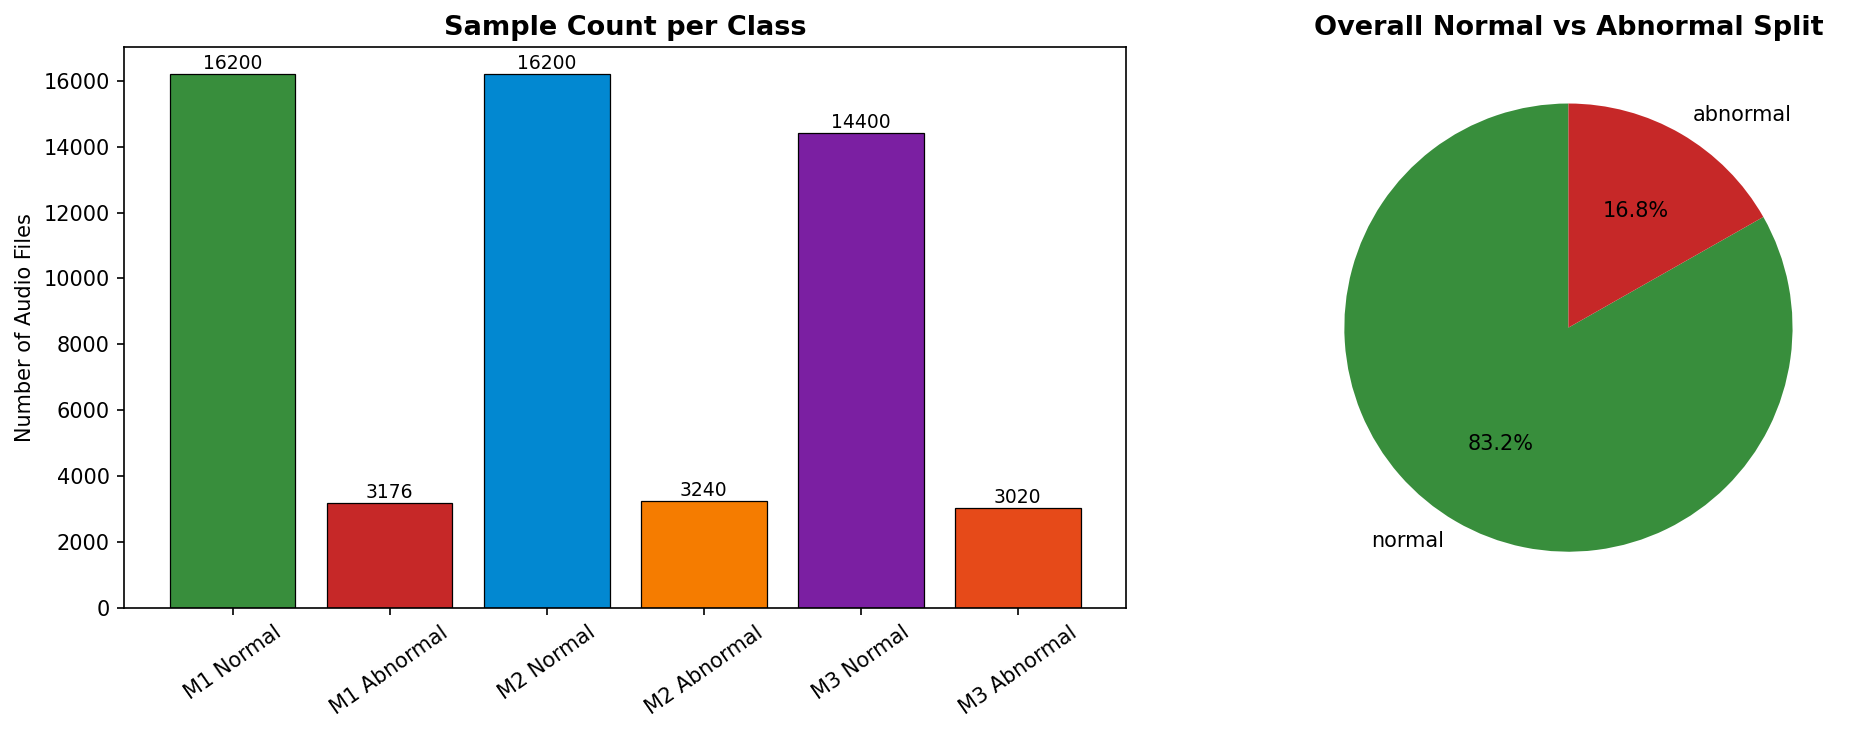
\includegraphics[width=0.7\textwidth]{figures/eda_class_balance.png}
    \caption{Class Balance across Machines 1, 2, and 3 (Normal vs. Abnormal)}
    \label{fig:class_dist}
\end{figure}

The dataset exhibits a consistent 5:1 ratio of Normal to Abnormal recordings across all three machines. This inherent class imbalance across the entire dataset is the primary factor that influenced our decision to prioritize the Macro F1-score as our evaluation metric.

\section{Temporal and Spectral Distributions}
Detailed metadata analysis confirms that 100\% of the dataset is recorded at a uniform sample rate of 48 kHz. However, audio durations are discrete and machine-dependent: Machine 1 and 2 are exactly 11.0 seconds, while Machine 3 is exactly 10.0 seconds. 

\begin{figure}[H]
    \centering
    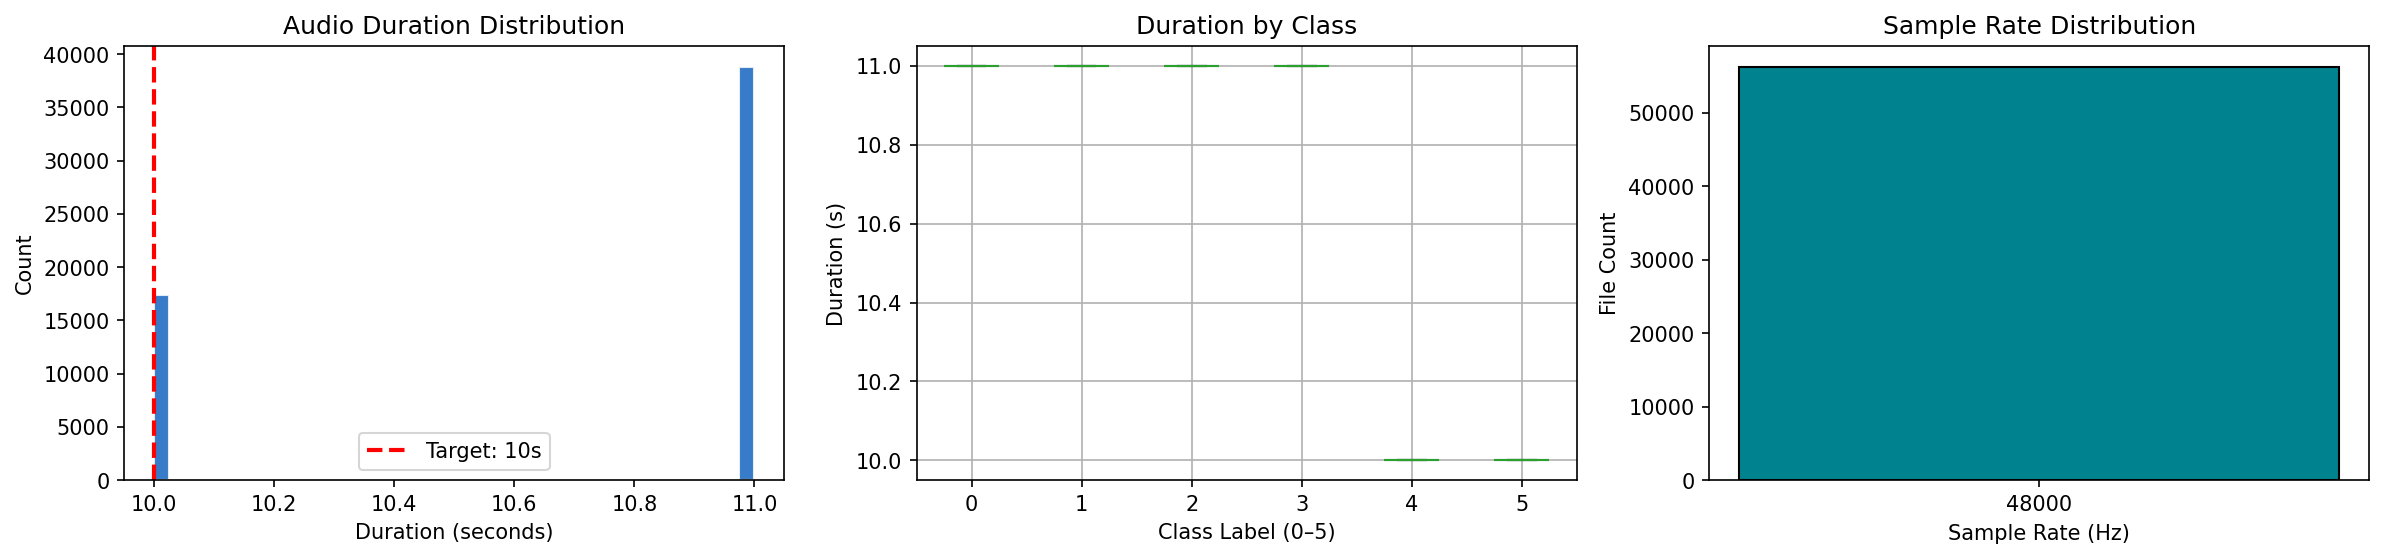
\includegraphics[width=0.7\textwidth]{figures/eda_duration_sr.png}
    \caption{Distribution of Recording Durations and Sample Rates}
    \label{fig:duration_sr}
\end{figure}

To handle this variability, our pipeline pads all recordings to a fixed 11-second window, ensuring that the critical "end-of-cycle" anomalies in Machines 1 and 2 are never truncated.

\section{Spectral and Waveform Comparison}
By comparing the raw waveforms and Mel-spectrograms of normal and abnormal recordings, we can identify visual patterns in the acoustic frequency domain. 

\begin{figure}[H]
    \centering
    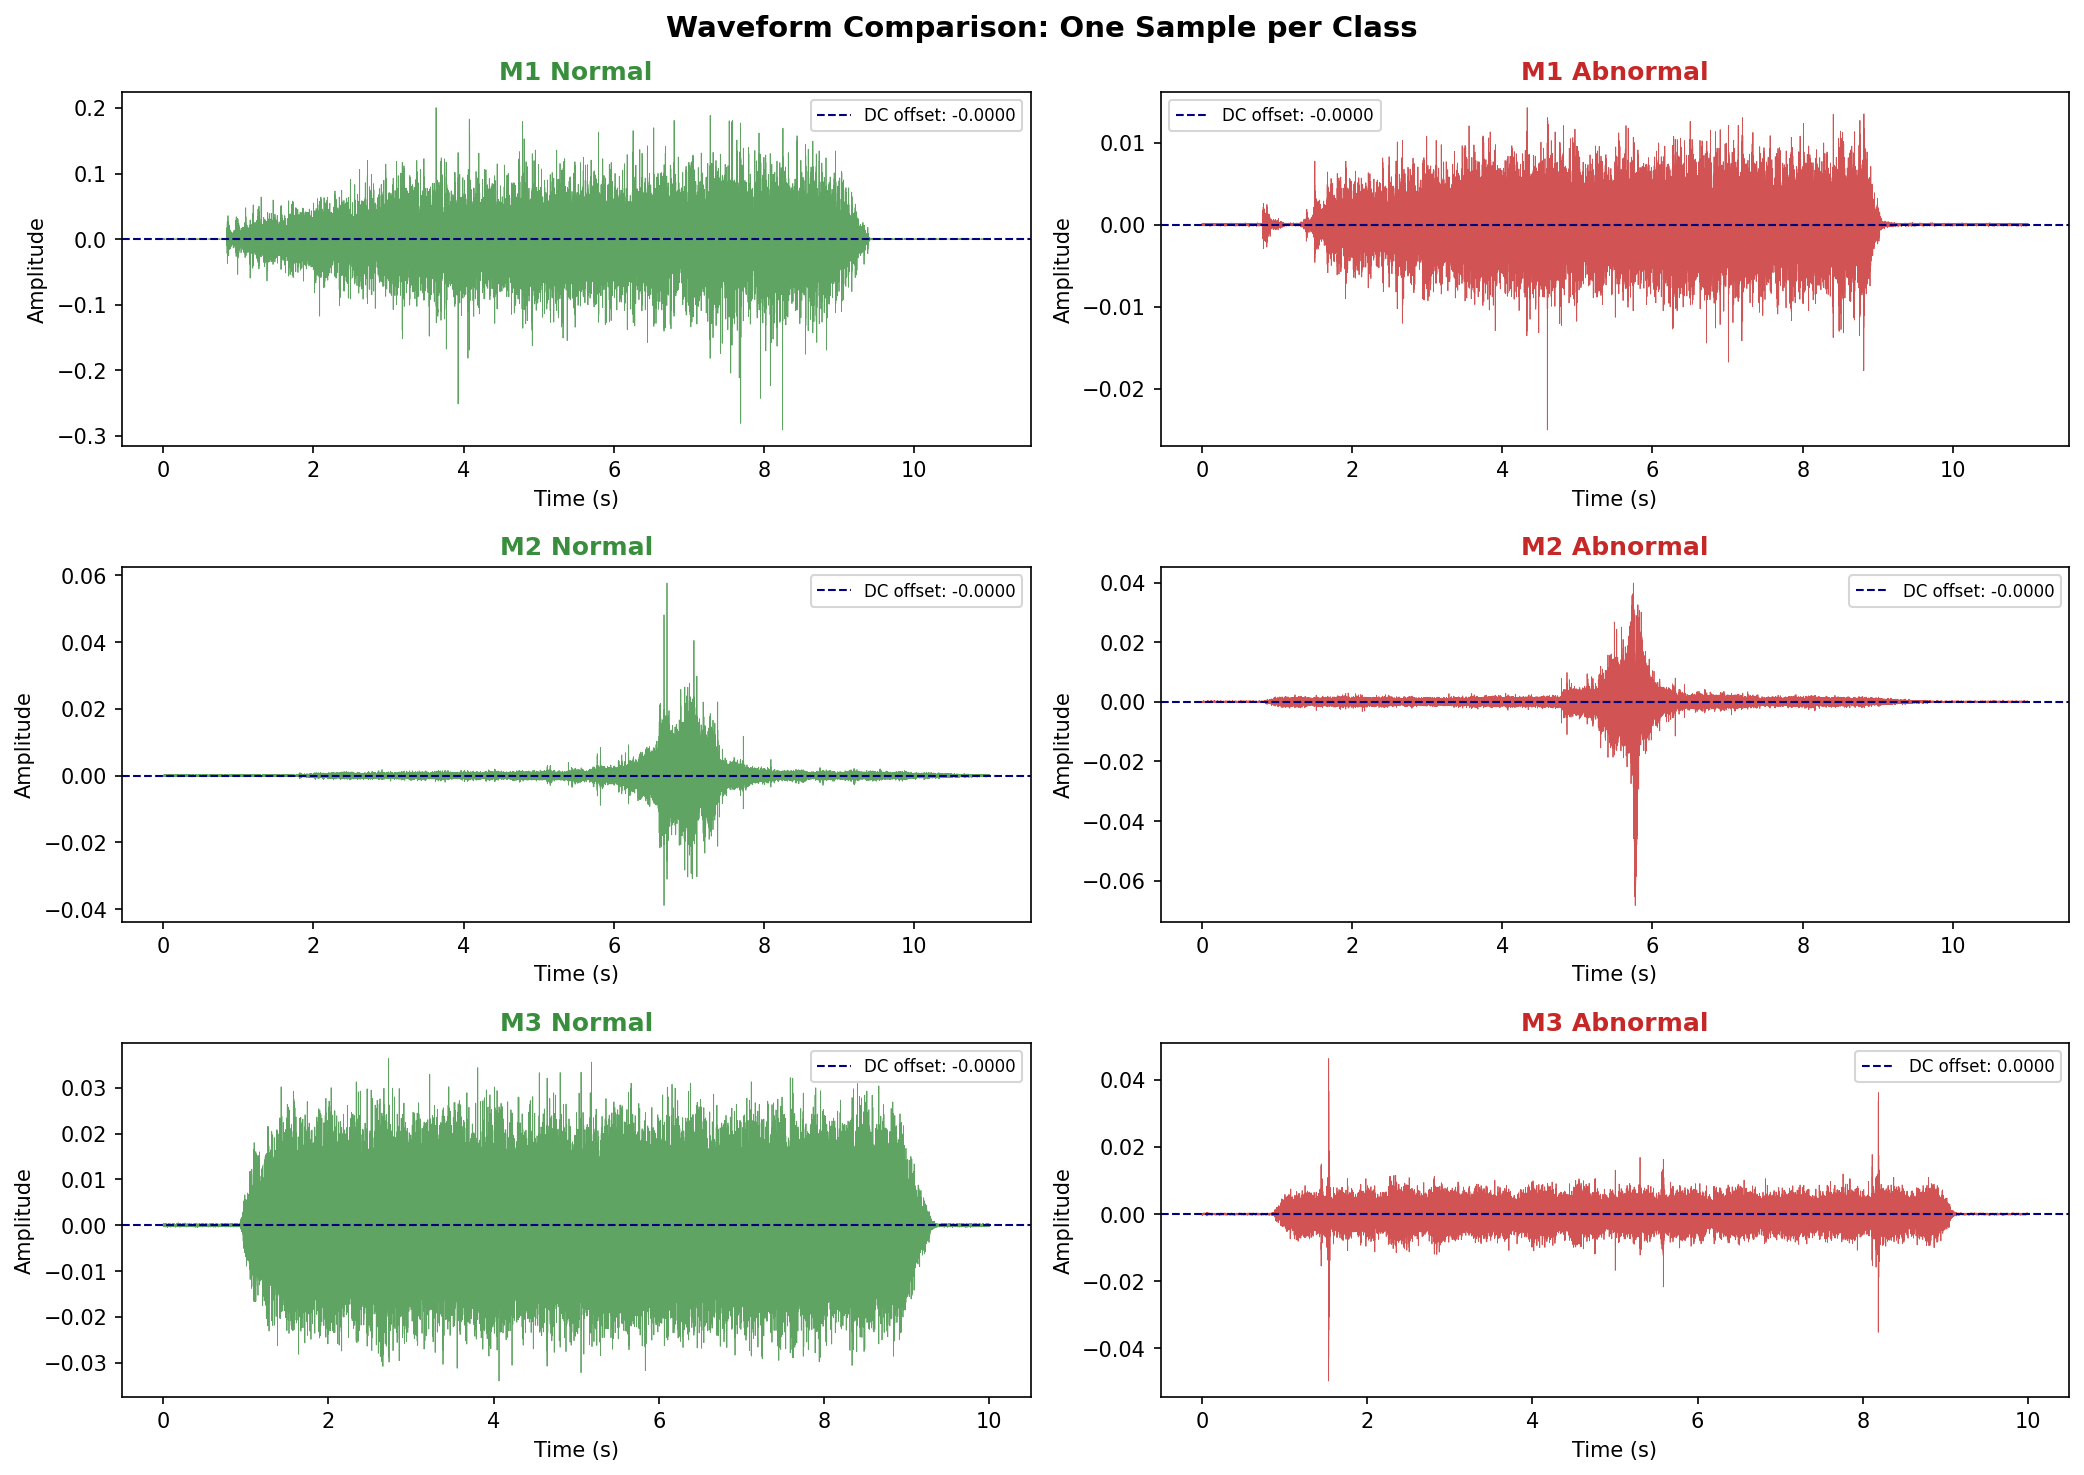
\includegraphics[width=0.75\textwidth]{figures/eda_waveforms.png}
    \caption{Time-Domain Waveform Comparison (Normal vs. Abnormal)}
    \label{fig:waveforms}
\end{figure}

\begin{figure}[H]
    \centering
    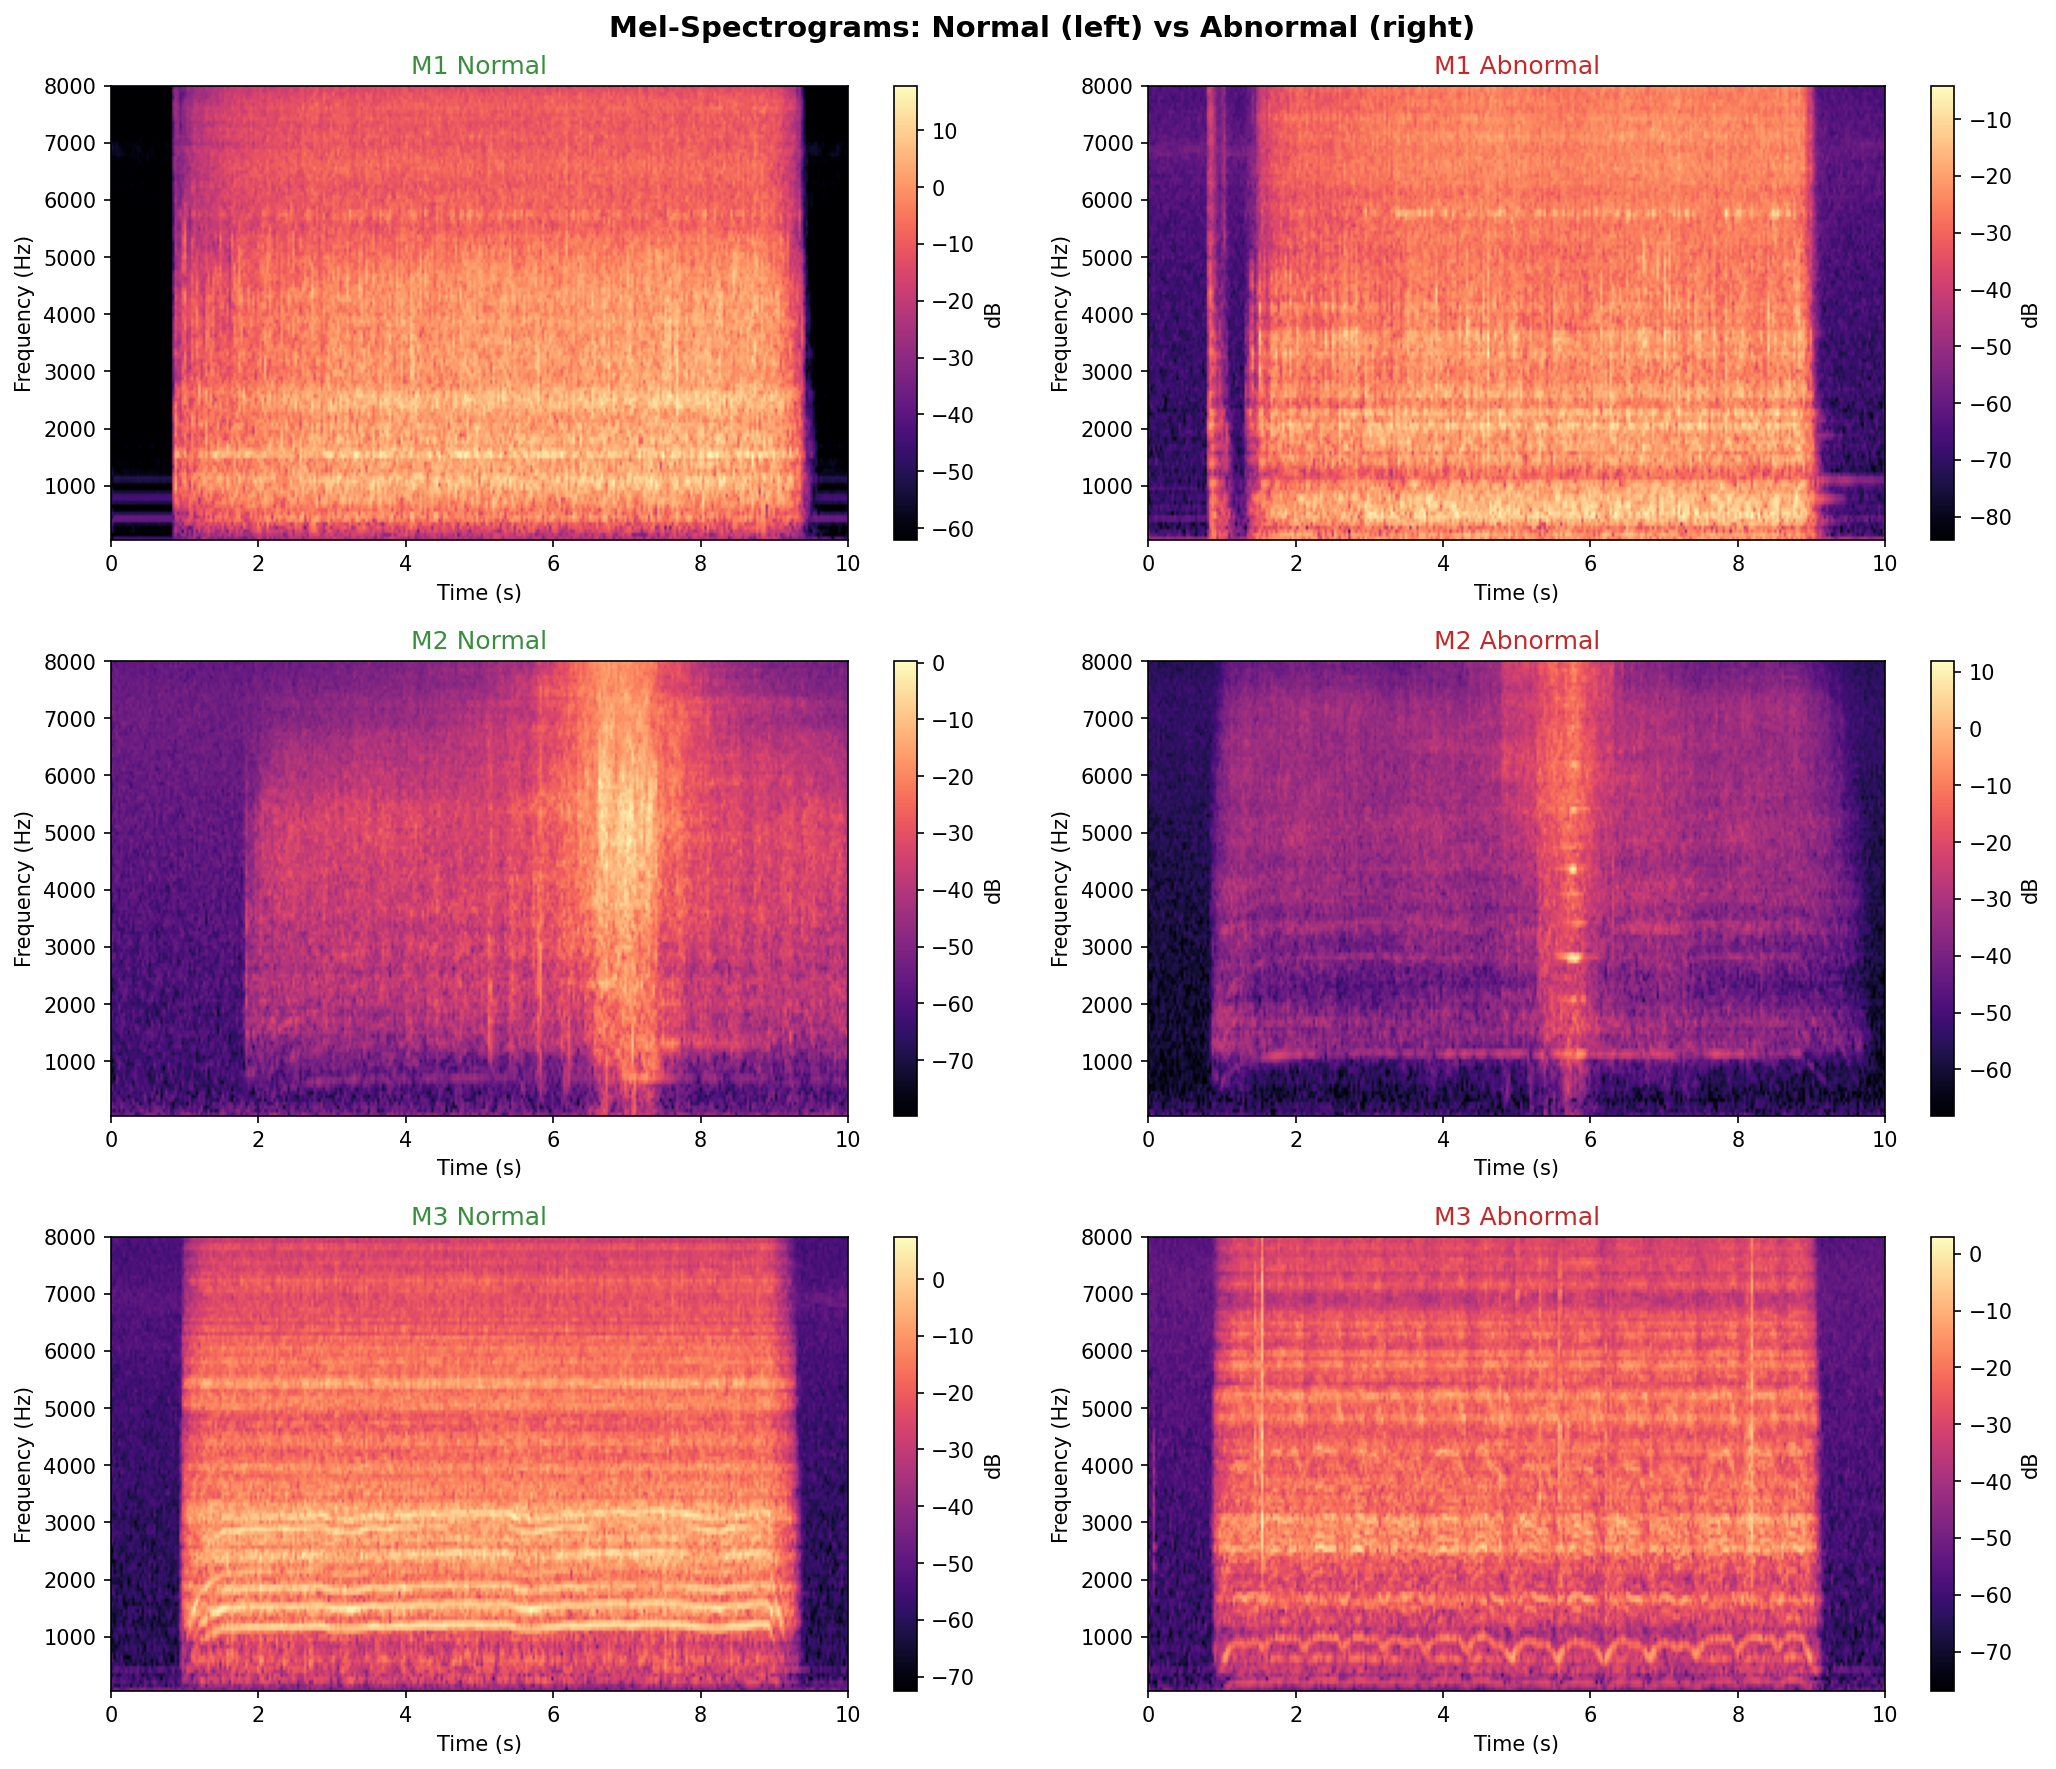
\includegraphics[width=0.75\textwidth]{figures/eda_spectrograms.png}
    \caption{Mel-Spectrogram Visual Signatures}
    \label{fig:spectrograms}
\end{figure}

\subsection{Normal Acoustic Signatures}
Normal recordings are characterized by stable, periodic harmonic structures. In Machines 1 and 2, the spectrogram shows consistent horizontal bands representing the fundamental frequency and its overtones, corresponding to constant rotation speeds.

\subsection{Abnormal Acoustic Signatures}
Anomalies often manifest as transient energy bursts or broadband noise. General patterns observed across the dataset include:
\begin{itemize}
    \item \textbf{Impulse Noise:} High-intensity vertical streaks indicating clashing components or gear teeth chipping.
    \item \textbf{Harmonic Shift:} Changes in the overtone structure, often indicating mechanical loose-fit or bearing degradation.
    \item \textbf{Signal-to-Noise Ratio (SNR) Drops:} Abnormal states frequently show a higher noise floor across all frequencies compared to normal states.
\end{itemize}

\begin{figure}[H]
    \centering
    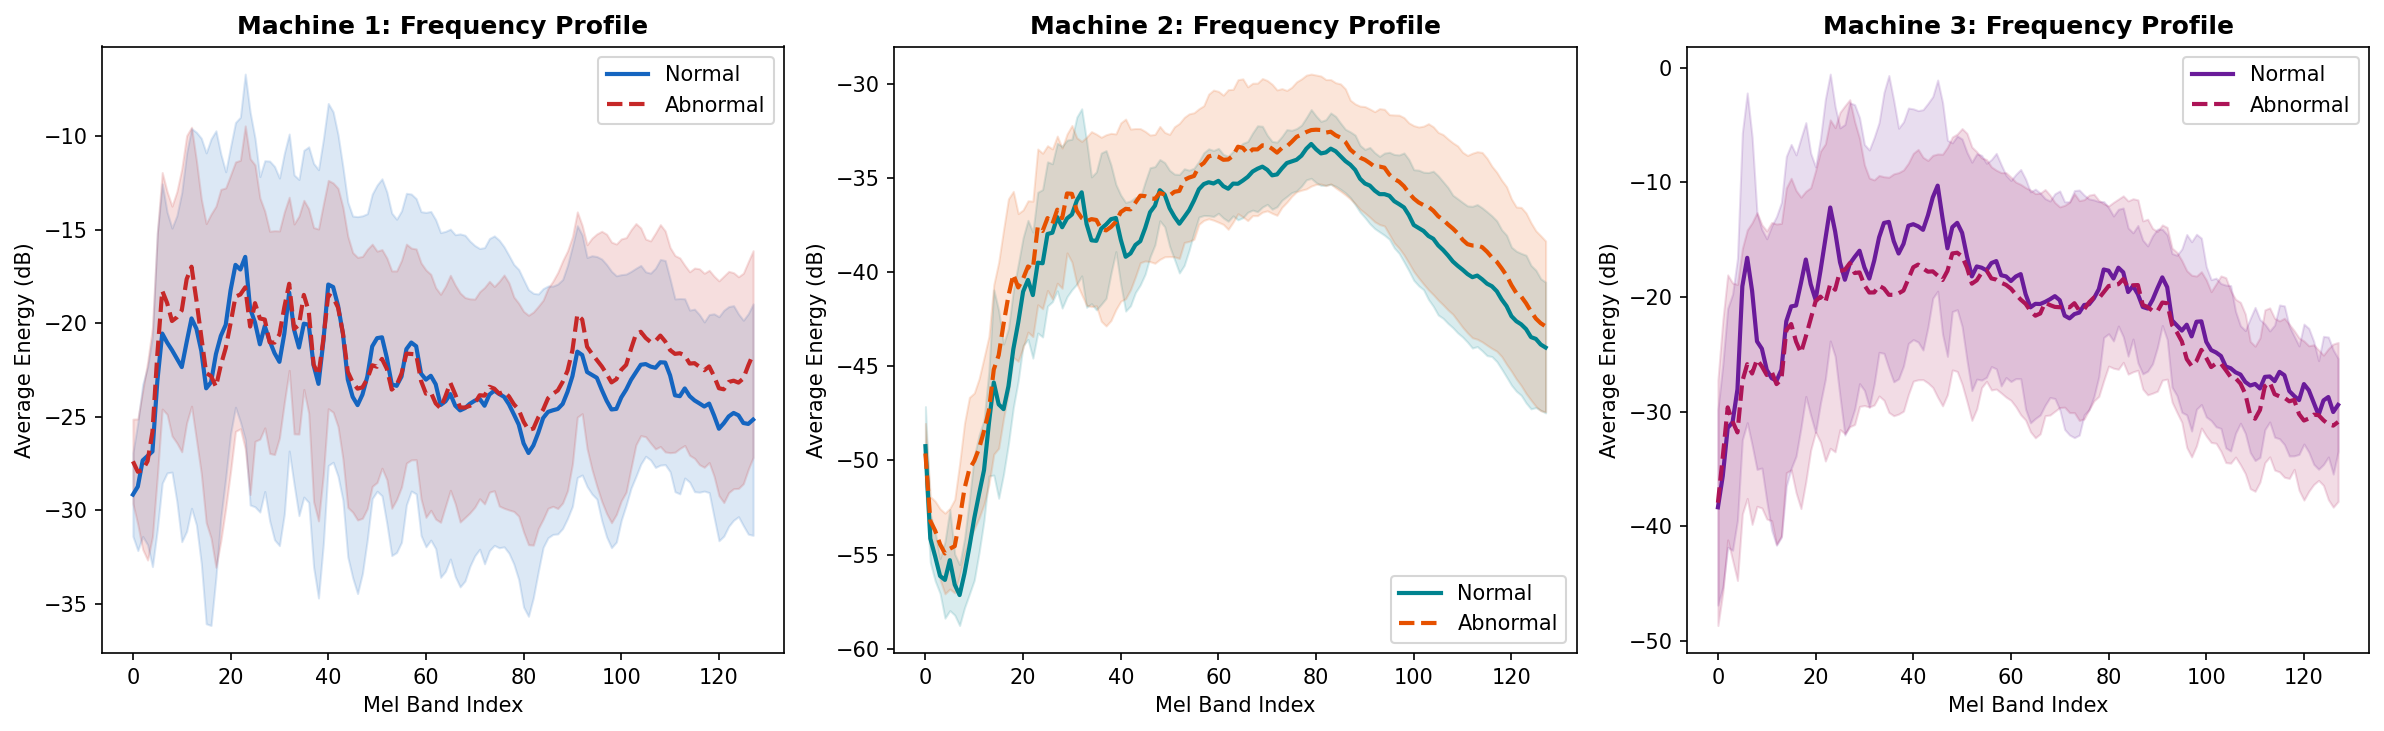
\includegraphics[width=0.8\textwidth]{figures/eda_freq_profiles.png}
    \caption{Frequency Band Profiles across Machines}
    \label{fig:freq_profiles}
\end{figure}

\begin{figure}[H]
    \centering
    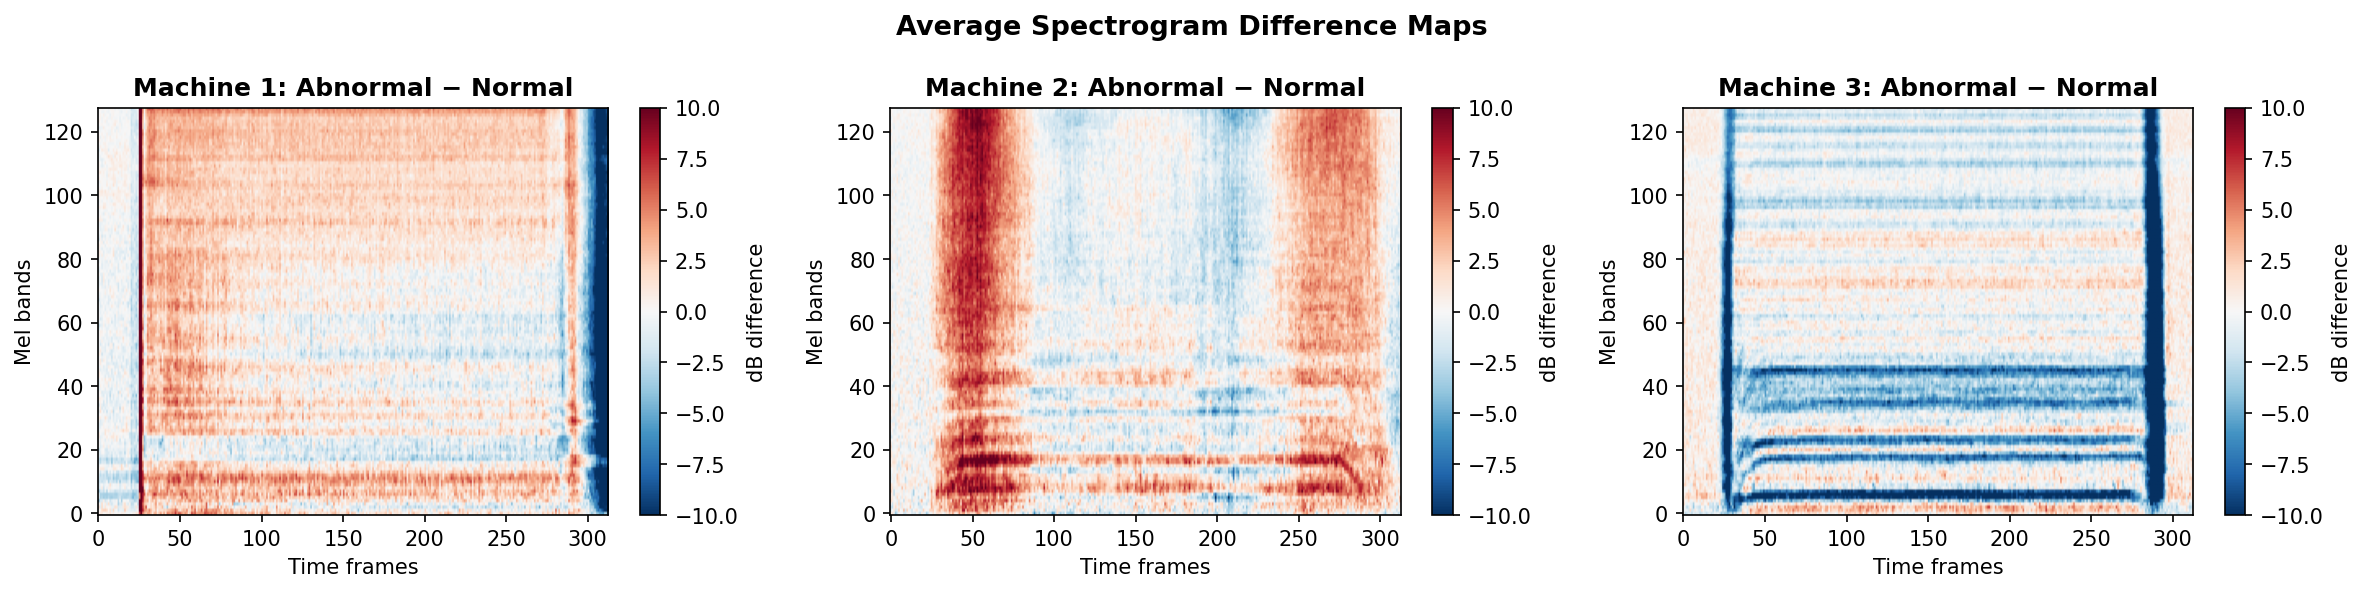
\includegraphics[width=0.8\textwidth]{figures/eda_diff_maps.png}
    \caption{Spectral Difference Maps (Abnormal - Normal)}
    \label{fig:diff_maps}
\end{figure}

\section{RMS Energy and Statistical Significance}
Mann-Whitney U Tests confirm that the difference in RMS Energy between Normal and Abnormal states is highly statistically significant ($p < 0.001$) across all machines. This justifies our decision to prohibit per-file normalization, as absolute volume is a critical feature.

\begin{figure}[H]
    \centering
    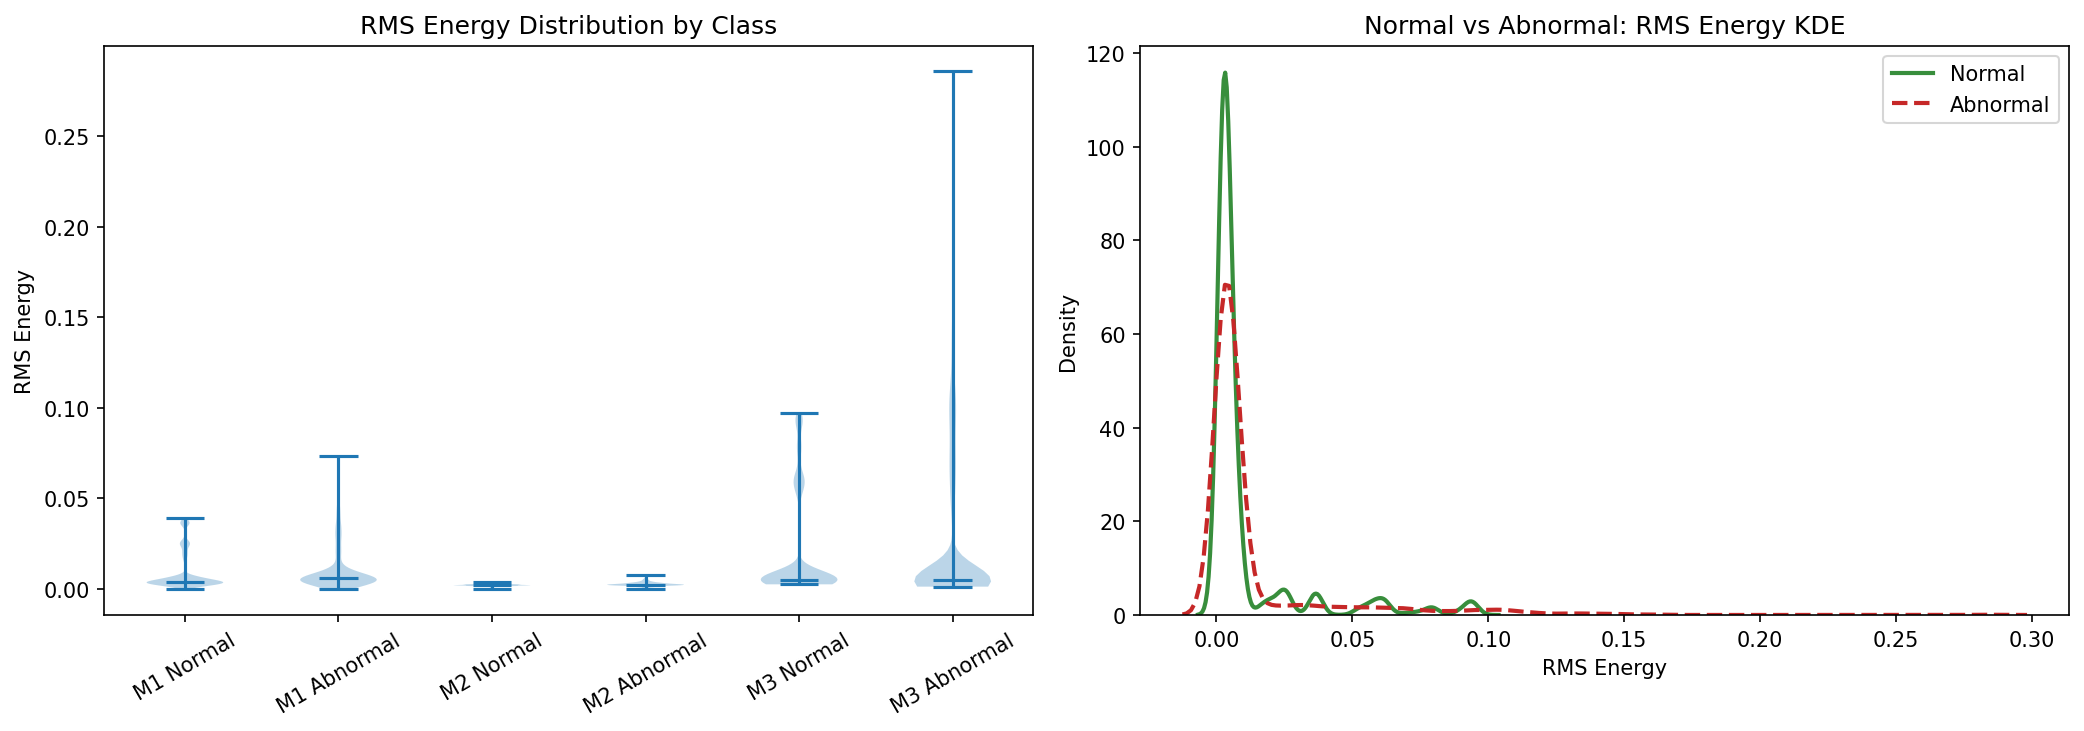
\includegraphics[width=0.7\textwidth]{figures/eda_energy.png}
    \caption{RMS Energy Distribution (Statistically Significant Separation)}
    \label{fig:energy_dist}
\end{figure}

\section{Outliers and Data Quality}
Exactly 142 files (0.3\% of the dataset) exhibited extreme energy z-scores > 3. These represent catastrophic mechanical faults that must be preserved for training rather than clipped as noise.

\begin{figure}[H]
    \centering
    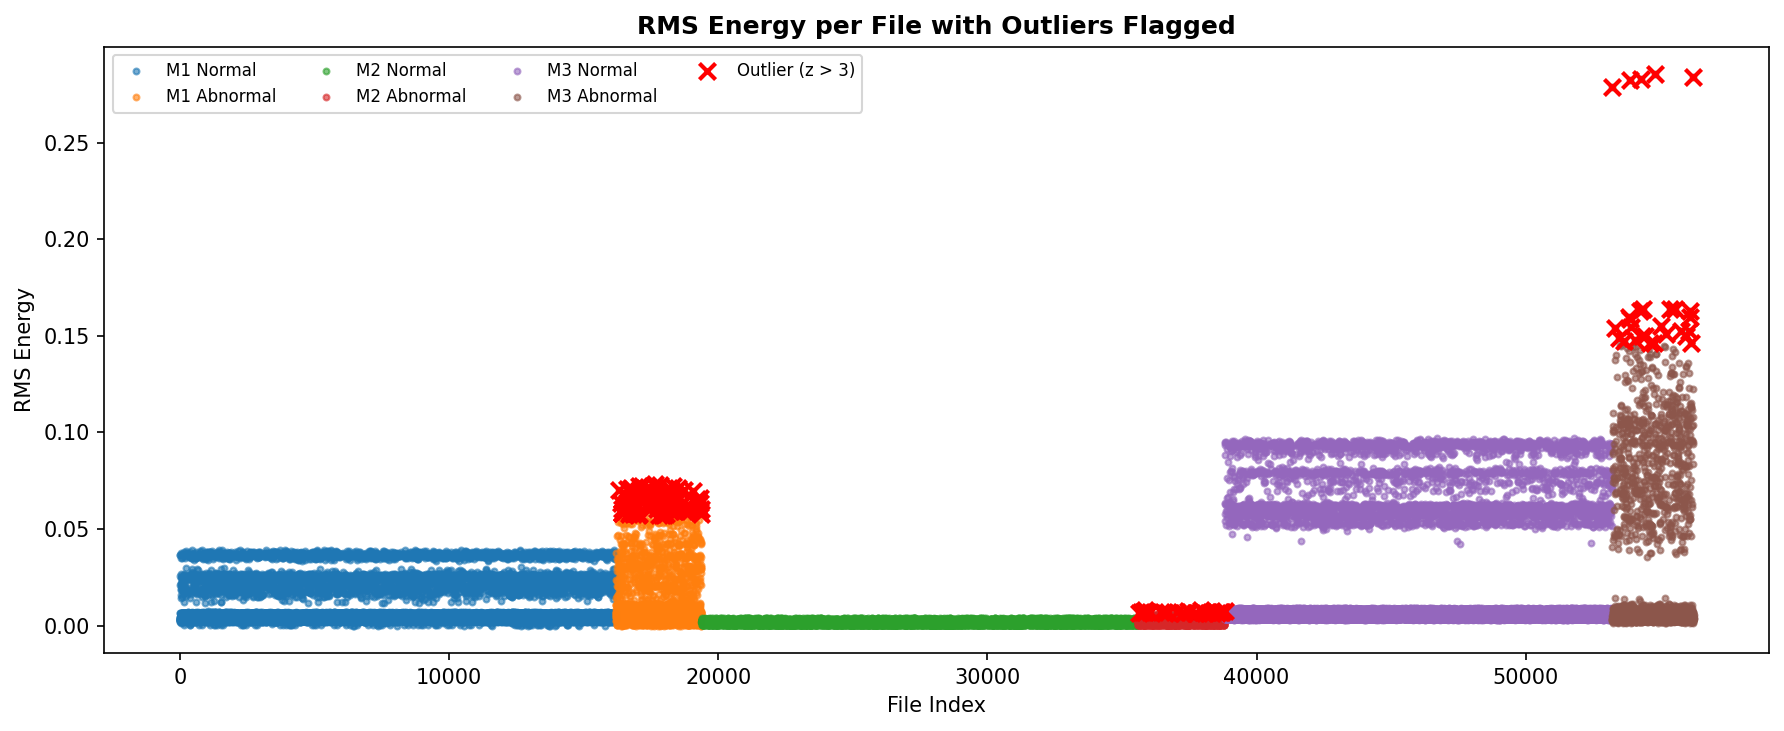
\includegraphics[width=0.7\textwidth]{figures/eda_outliers.png}
    \caption{Identification of High-Energy Acoustic Outliers}
    \label{fig:outliers}
\end{figure}

\section{Silence Ratio and Background Noise}
The dataset exhibits a high overall silence ratio (mean = 0.86), particularly in Machine 2. This confirms that anomalies are highly localized in time, necessitating the use of temporal attention in our Deep Learning architecture.

\begin{figure}[H]
    \centering
    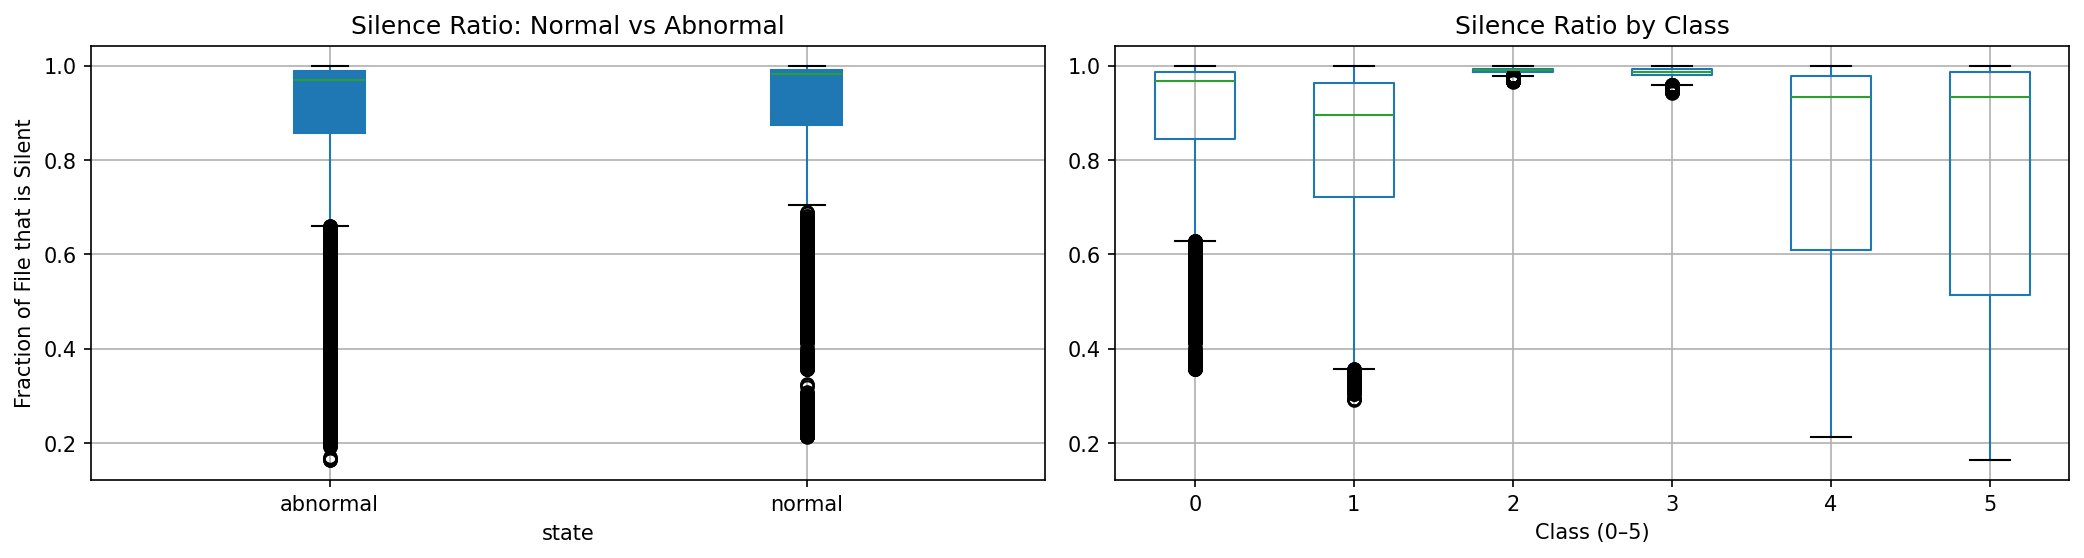
\includegraphics[width=0.7\textwidth]{figures/eda_silence.png}
    \caption{Silence Ratio Analysis across Machine States}
    \label{fig:silence_ratio}
\end{figure}

\section{Correlation Analysis}
We conducted a correlation analysis of basic acoustic features. We found that abnormal samples often have a higher Zero-Crossing Rate (ZCR) due to the increased mechanical noise and clatter associated with faults.

\section{High-Dimensional Visualization (t-SNE)}
To evaluate the inherent separability of the 100 extracted features, we employed t-Distributed Stochastic Neighbor Embedding (t-SNE). This non-linear dimensionality reduction technique allows us to visualize high-dimensional clusters in a 2D space while preserving local structures.

\begin{figure}[H]
    \centering
    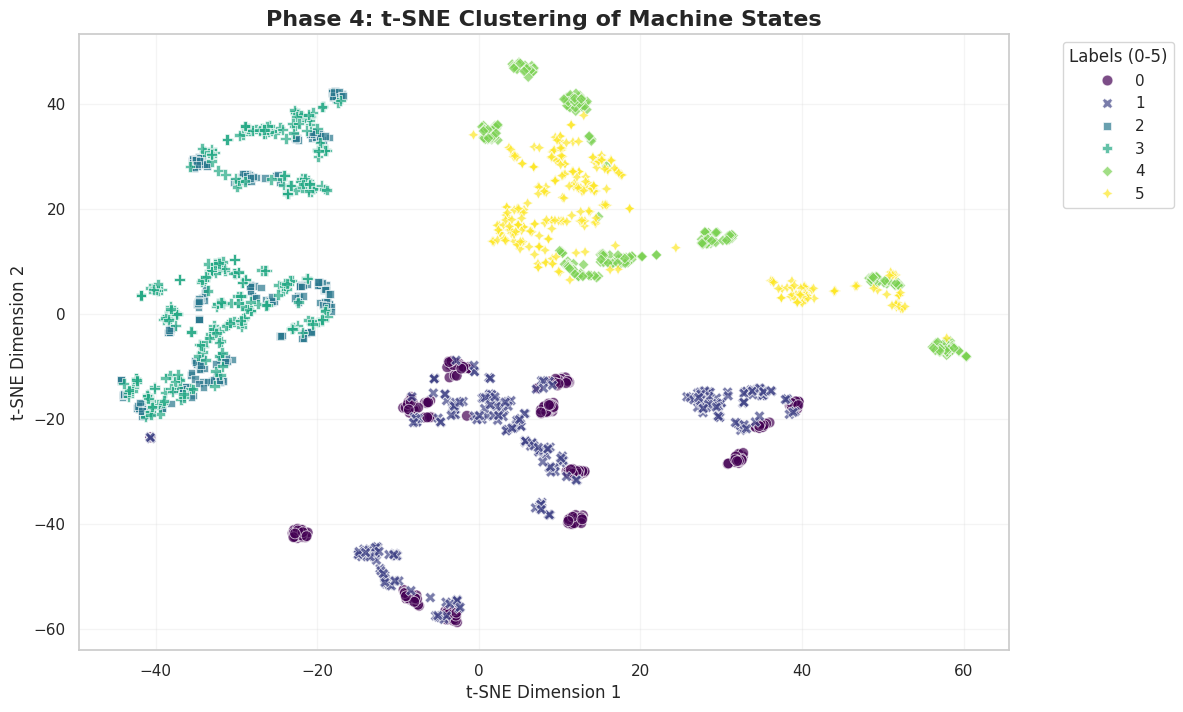
\includegraphics[width=0.8\textwidth]{figures/notebook_tsne_plot.png}
    \caption{t-SNE Projection of Acoustic Features across 6 Classes}
    \label{fig:tsne_plot}
\end{figure}

The t-SNE plot revealed distinct macro-clusters corresponding to each of the three machines, indicating that a machine's baseline mechanical signature is the most dominant acoustic feature. Crucially, within each machine-specific "island," the "Normal" and "Abnormal" samples exhibit clear sub-clustering and separation. This confirms that the hand-crafted acoustic manifold successfully captures both machine identity and fault status.

\section{Feature Inter-correlation}
Correlation heatmaps of the Top 15 features showed that while MFCCs are highly correlated with each other, Spectral Contrast and Zero-Crossing Rate provide independent information. This low inter-correlation between diverse feature families is why our hand-crafted acoustic manifold achieves high performance.

\begin{figure}[H]
    \centering
    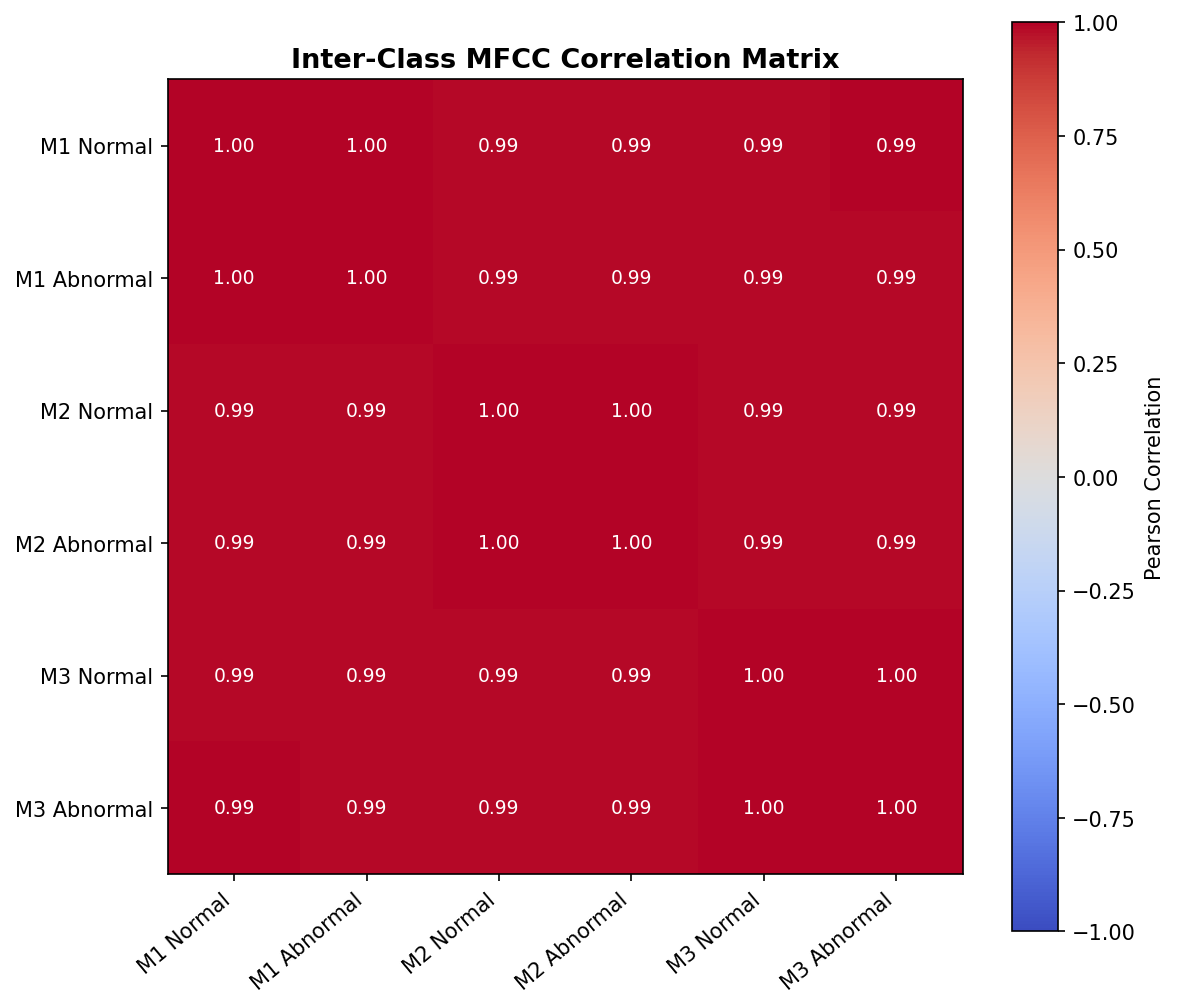
\includegraphics[width=0.7\textwidth]{figures/eda_correlation.png}
    \caption{Correlation Heatmap of Top Acoustic Features}
    \label{fig:corr_heatmap}
\end{figure}

\section{Machine-Specific Distinctions}
Boxplot analysis across Machines 1, 2, and 3 showed that while the absolute values of Spectral Centroid vary significantly between machines (due to different motor speeds), the \textit{relative shift} between Normal and Abnormal states remains consistent, providing a robust signature for anomaly detection.

\begin{figure}[H]
    \centering
    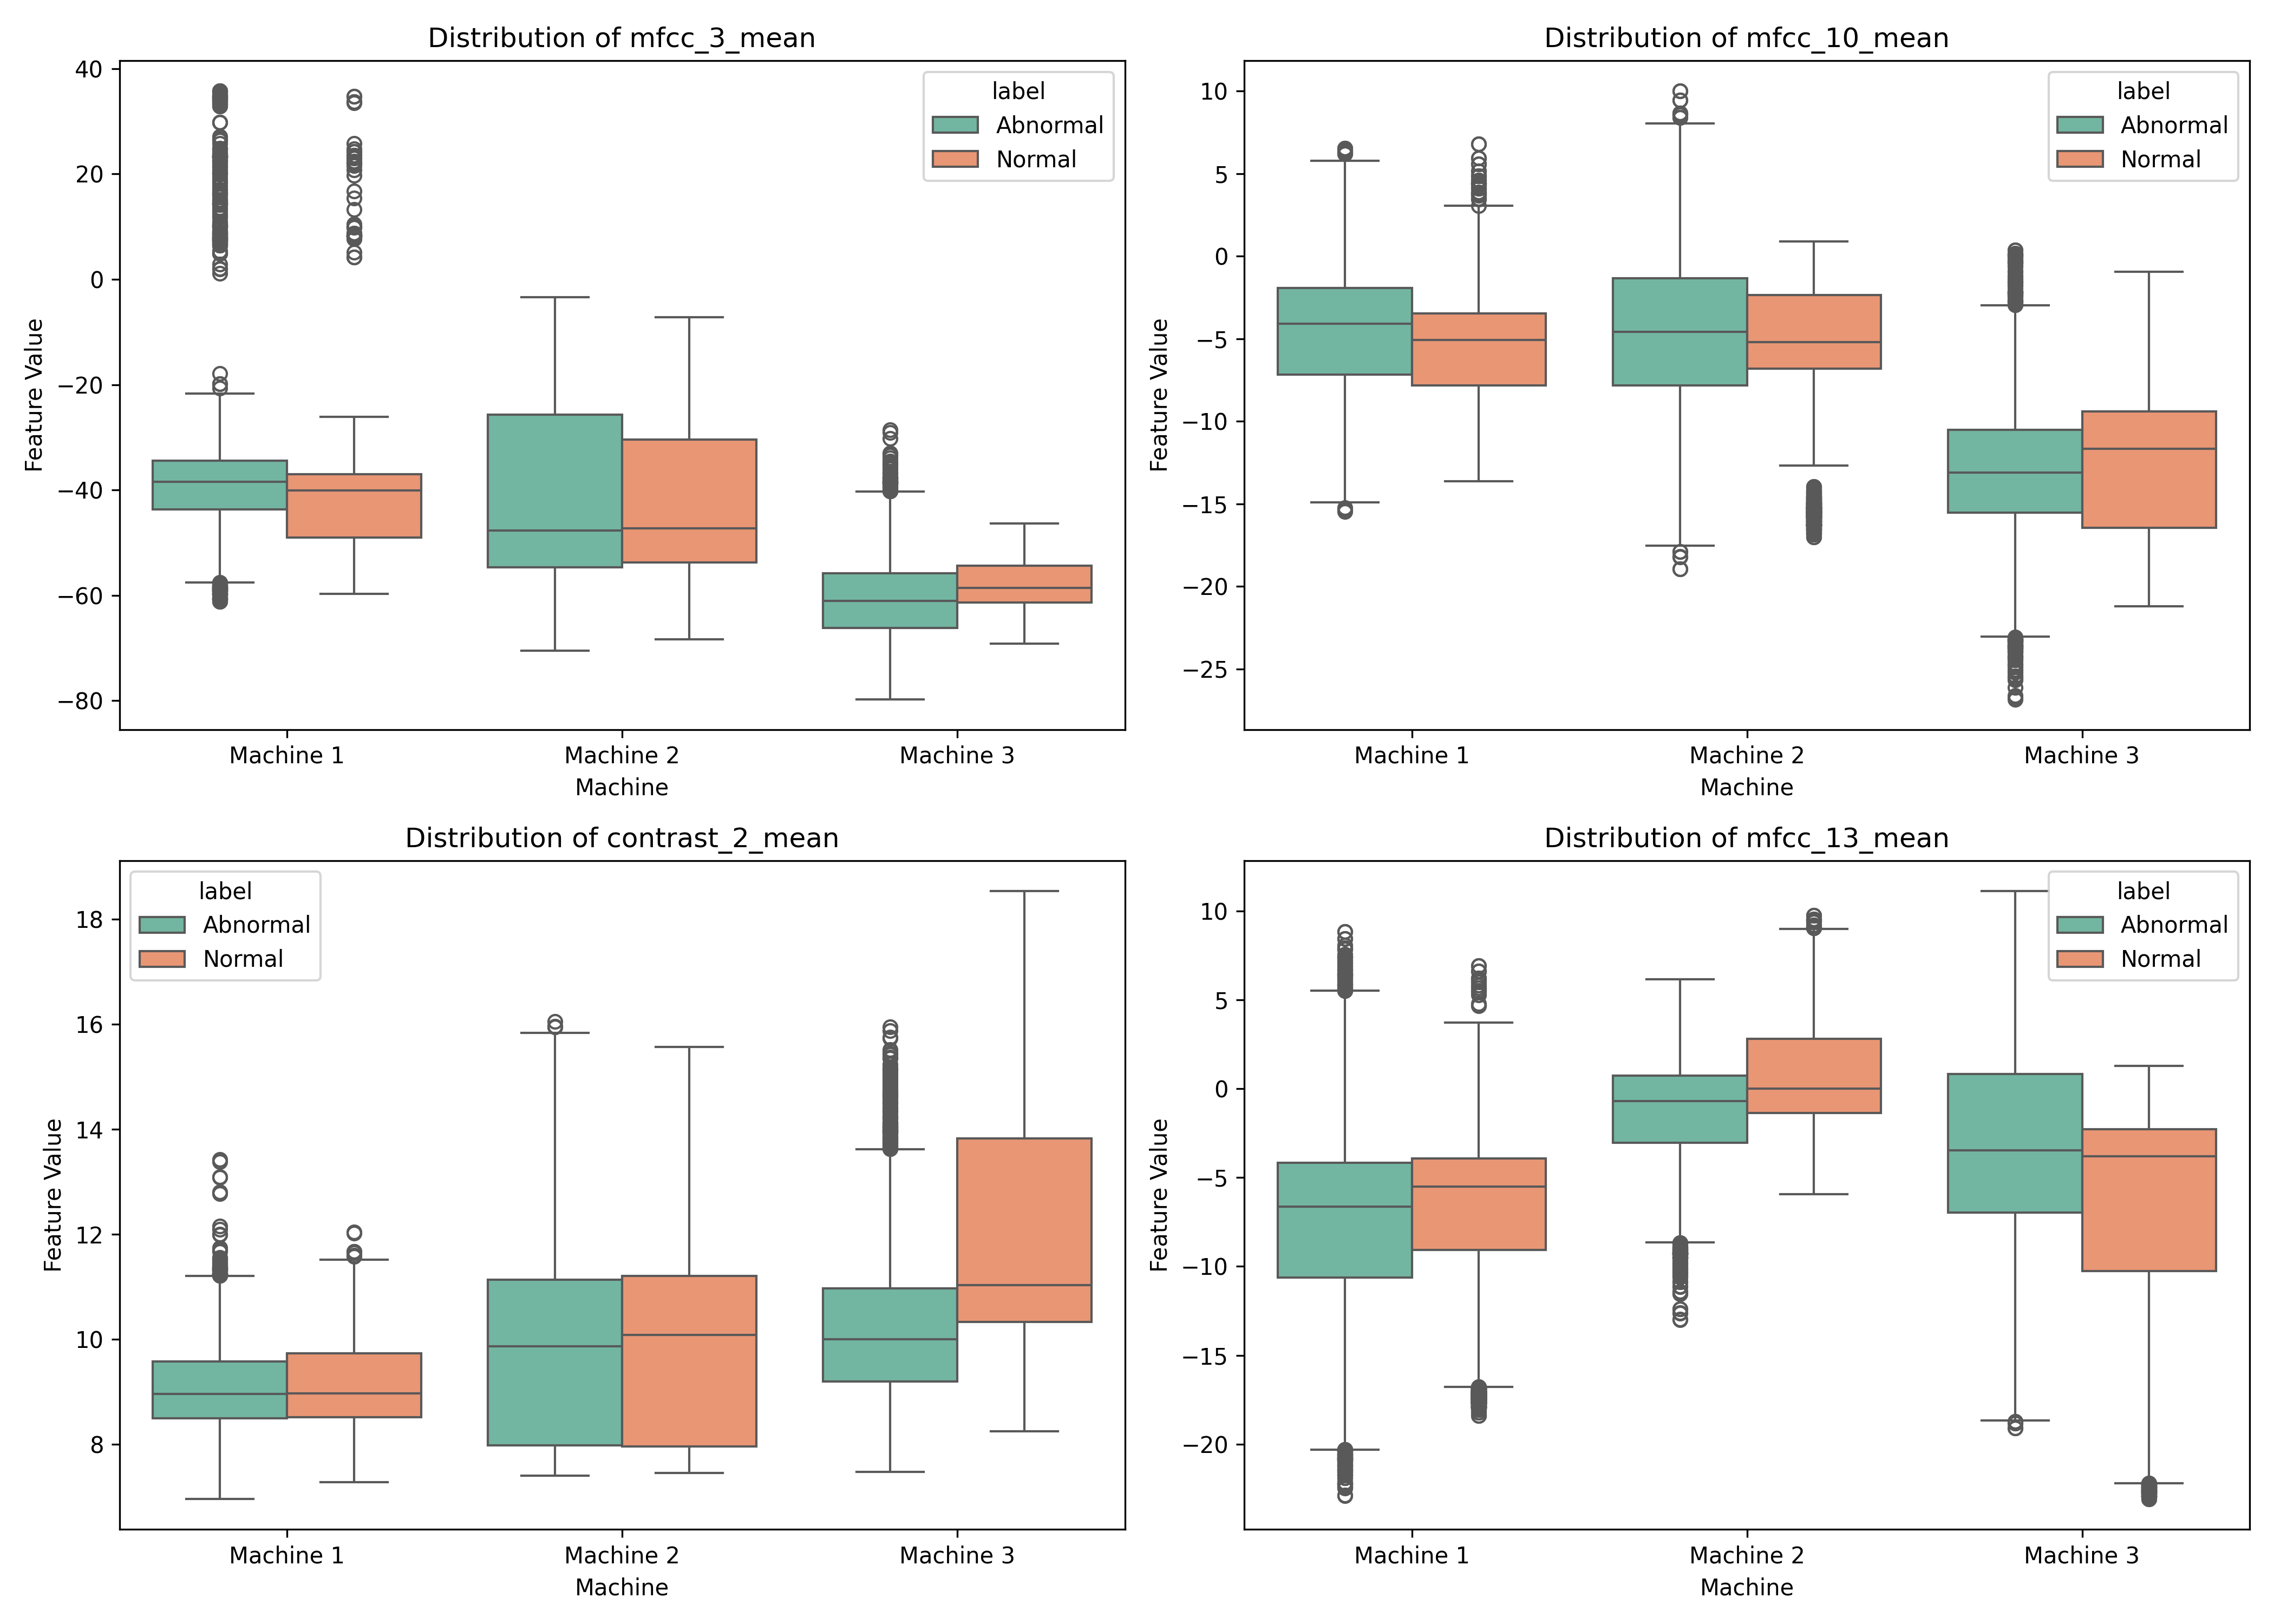
\includegraphics[width=0.7\textwidth]{figures/top_features_boxplot.png}
    \caption{Distribution of Top 4 Features across Machines}
    \label{fig:top_features_boxplot}
\end{figure}

\chapter{Feature Engineering}

\section{The Acoustic Manifold}
The core of our tabular modeling approach is the extraction of a 100-dimensional feature vector from the raw audio signal. This "Acoustic Manifold" captures the mathematical representation of the sound across time, frequency, and harmonic domains. The 100 features are derived from 25 base acoustic metrics, each expanded by four statistical moments: mean, standard deviation, maximum, and minimum.

\section{Feature Categories}

\subsection{Mel-Frequency Cepstral Coefficients (MFCCs)}
MFCCs are the standard in audio processing, representing the short-term power spectrum of a sound. We extracted 13 MFCC coefficients, providing a detailed view of the spectral envelope. For each coefficient, we computed:
\begin{itemize}
    \item \textbf{Statistical Expansion:} Mean, standard deviation, maximum, and minimum values across the time-axis, resulting in 52 MFCC-based features.
\end{itemize}

\subsection{Spectral Shape Features}
Beyond MFCCs, we extracted several critical spectral metrics, each expanded with the same four statistical moments (12 features total):
\begin{itemize}
    \item \textbf{Spectral Centroid:} Indicates where the "center of mass" of the spectrum is located (related to brightness).
    \item \textbf{Spectral Bandwidth:} Describes the range of frequencies the signal covers.
    \item \textbf{Spectral Rolloff:} The frequency below which 85\% of the spectral power is concentrated.
\end{itemize}

\subsection{Spectral Contrast}
Spectral Contrast measures the difference in power between peaks and valleys across 7 frequency bands. This feature is expanded into 28 statistical columns and has proven highly effective for mechanical anomaly detection by capturing harmonic shifts.

\subsection{Temporal Features}
The time-domain characteristics are captured by 8 features (2 metrics $\times$ 4 stats):
\begin{itemize}
    \item \textbf{Zero-Crossing Rate (ZCR):} Captures the frequency at which the signal changes sign. High ZCR is often associated with high-frequency mechanical noise.
    \item \textbf{RMS Energy:} Measures the overall power/loudness of the recording.
\end{itemize}
All temporal features are likewise expanded into mean, std, max, and min statistics to capture both global properties and transient peaks.

\section{Feature Importance and Pruning}
To optimize for edge-deployment (where memory and CPU cycles are limited), we conducted a feature importance study using a Random Forest model with 50 estimators. 

\begin{figure}[H]
    \centering
    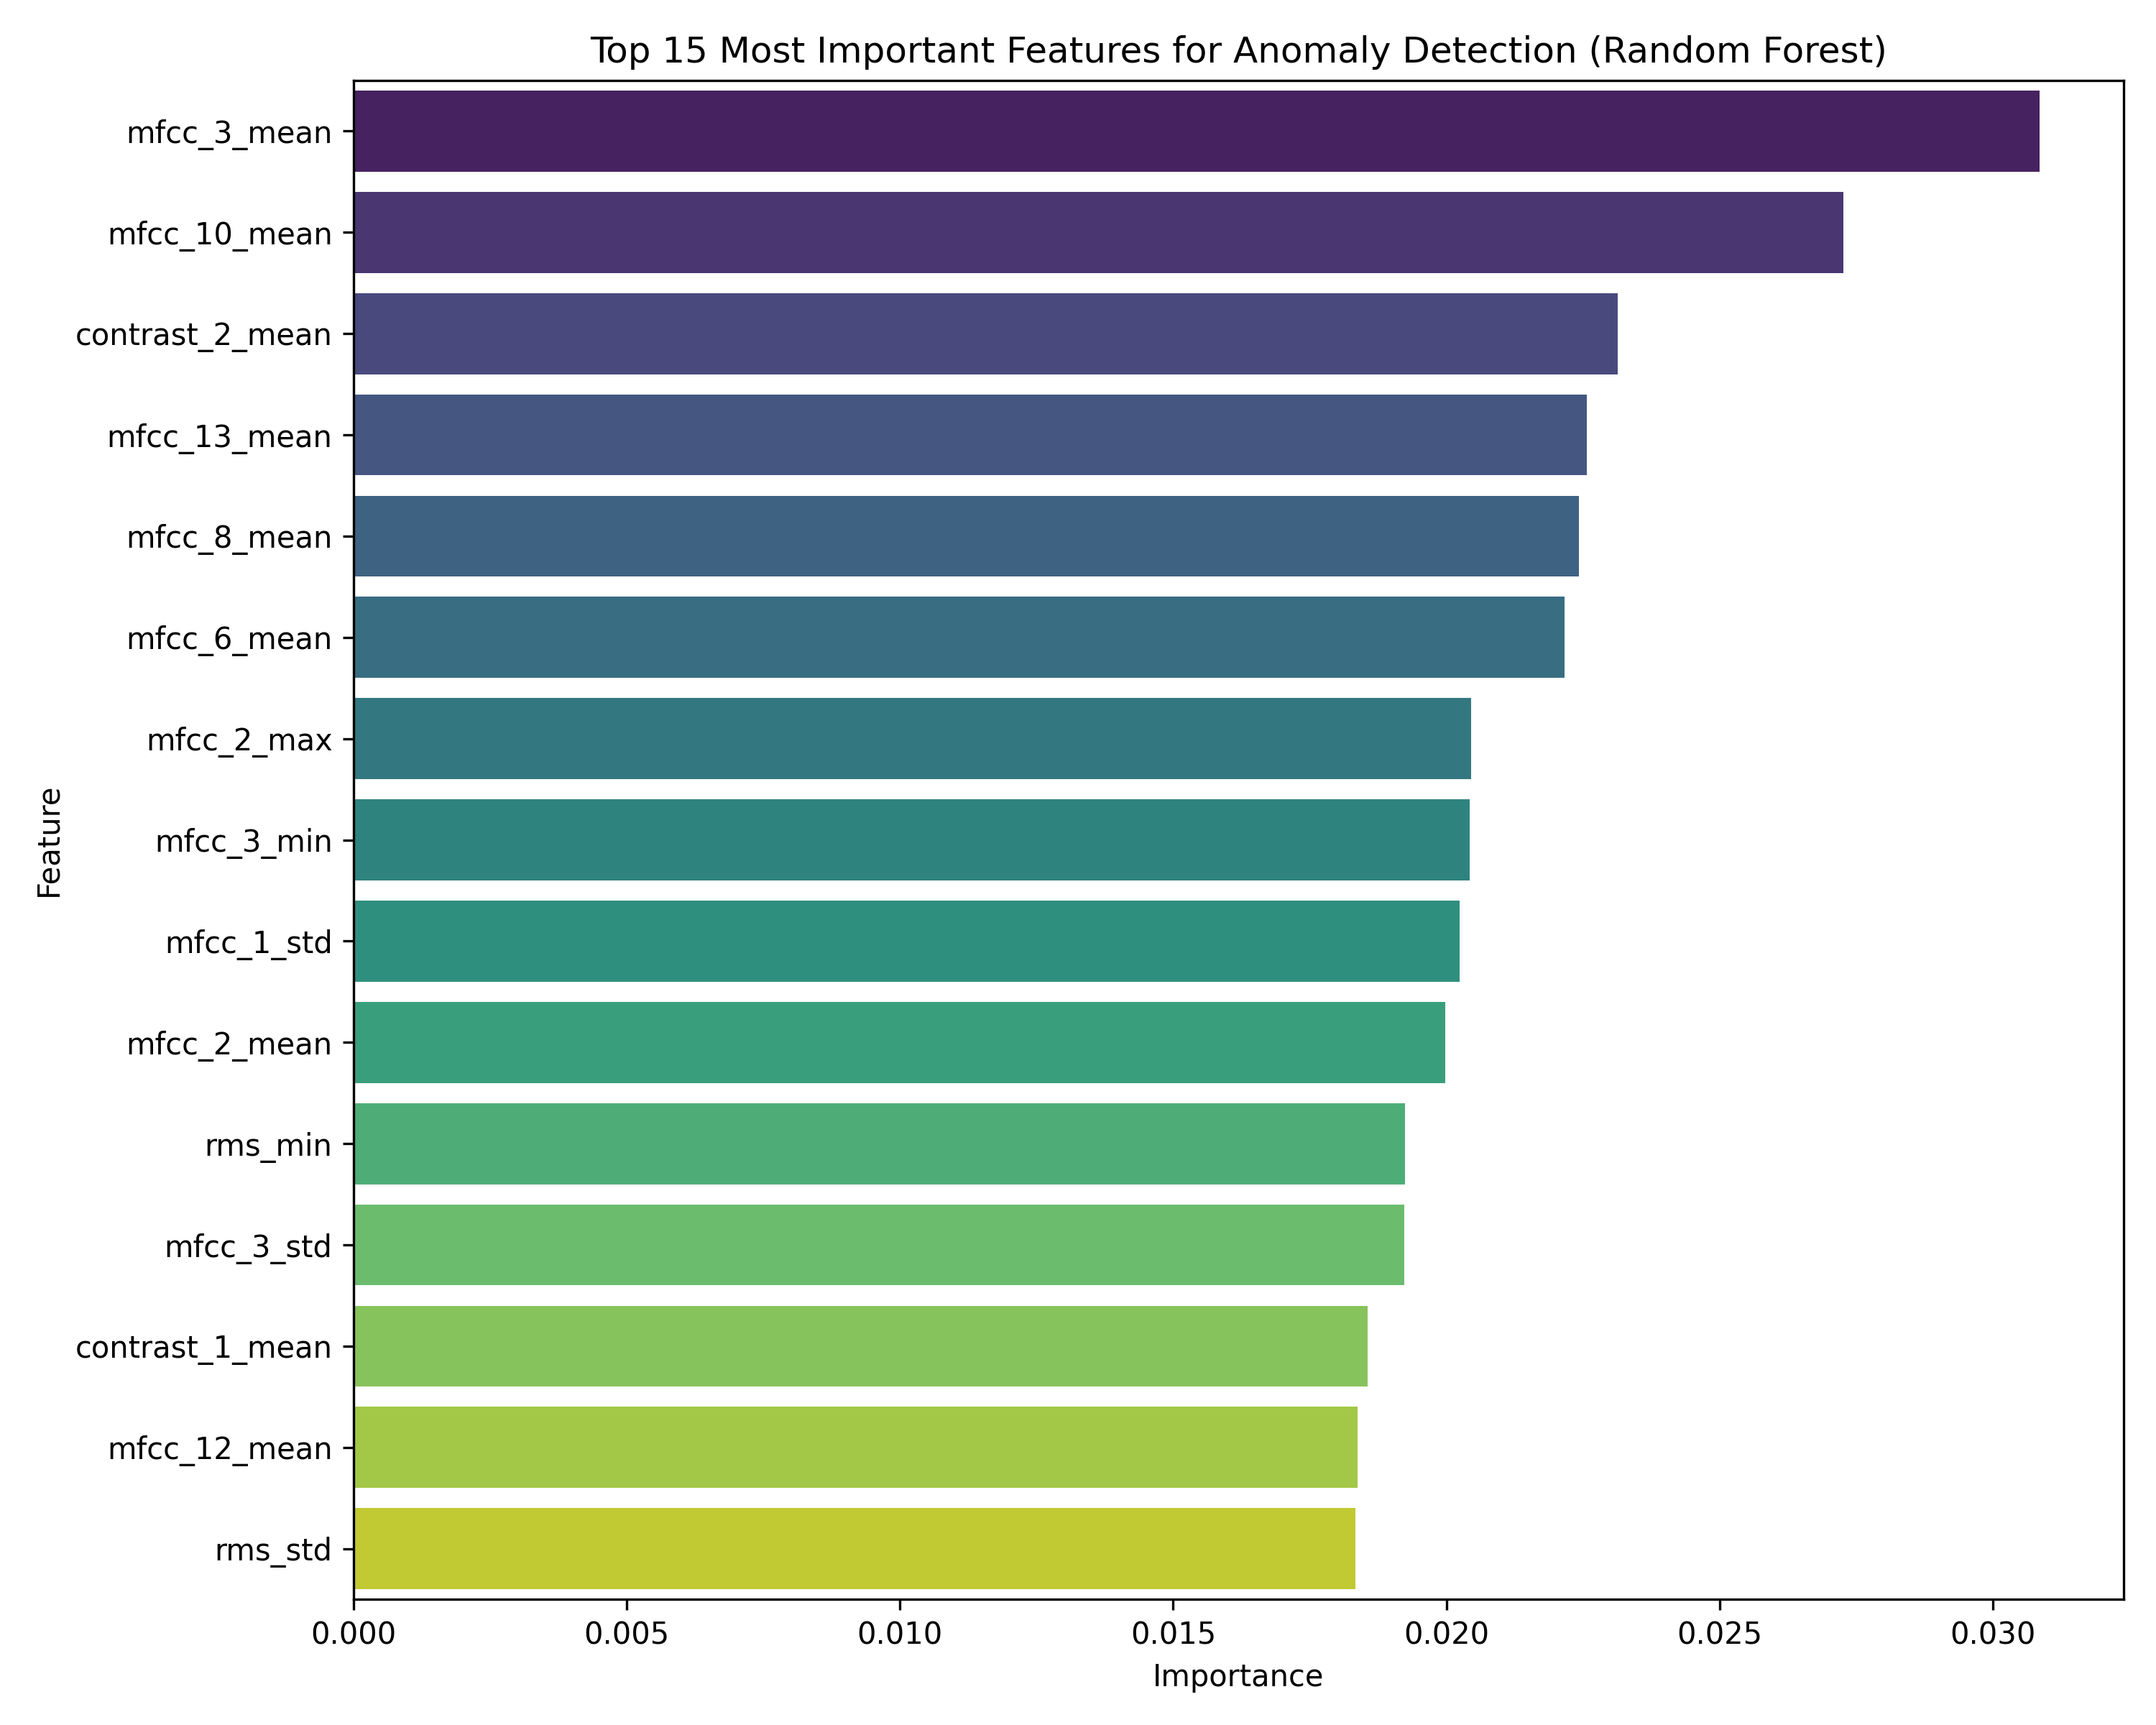
\includegraphics[width=0.8\textwidth]{figures/feature_importance.png}
    \caption{Top 20 Most Predictive Acoustic Features}
    \label{fig:feat_imp}
\end{figure}

By retaining only the Top 40 features, we were able to reduce the model size significantly while maintaining a high F1-score. This pruning process is essential for deploying the model on low-power industrial gateways.

\section{Normalization and Scaling}
Before training, all features are passed through a \texttt{StandardScaler} to ensure they have zero mean and unit variance. This step is critical for algorithms like SVM and Deep Learning, though less impactful for the gradient-boosted trees used in our final XGBoost model.

\chapter{Clustering and Overfitting Analysis}

\section{The Data Leakage Problem}
In many audio datasets, multiple segments are recorded from the same machine in a single session. These segments are highly correlated. If a standard random split is used, segments from the same session appear in both the training and test sets. 

The model effectively "memorizes" the unique background hum or specific microphone noise of that session and uses it to identify the machine, rather than learning generalizable fault indicators. This leads to artificially high accuracy scores (~99\%) that vanish when the model is tested on truly new machinery.

\section{Intra-Class Clustering Strategy}
To solve this, we implemented a clustering-aware splitting strategy. By grouping similar recordings within each class using K-Means, we created "Acoustic Groups."

\subsection{K-Means Clustering}
For each of the six classes, we run K-Means on the acoustic feature vectors. Each sample is assigned a Cluster ID. During cross-validation, we use \texttt{GroupKFold}, ensuring that all samples from a specific cluster are either entirely in the training set or entirely in the validation set.

\begin{figure}[H]
    \centering
    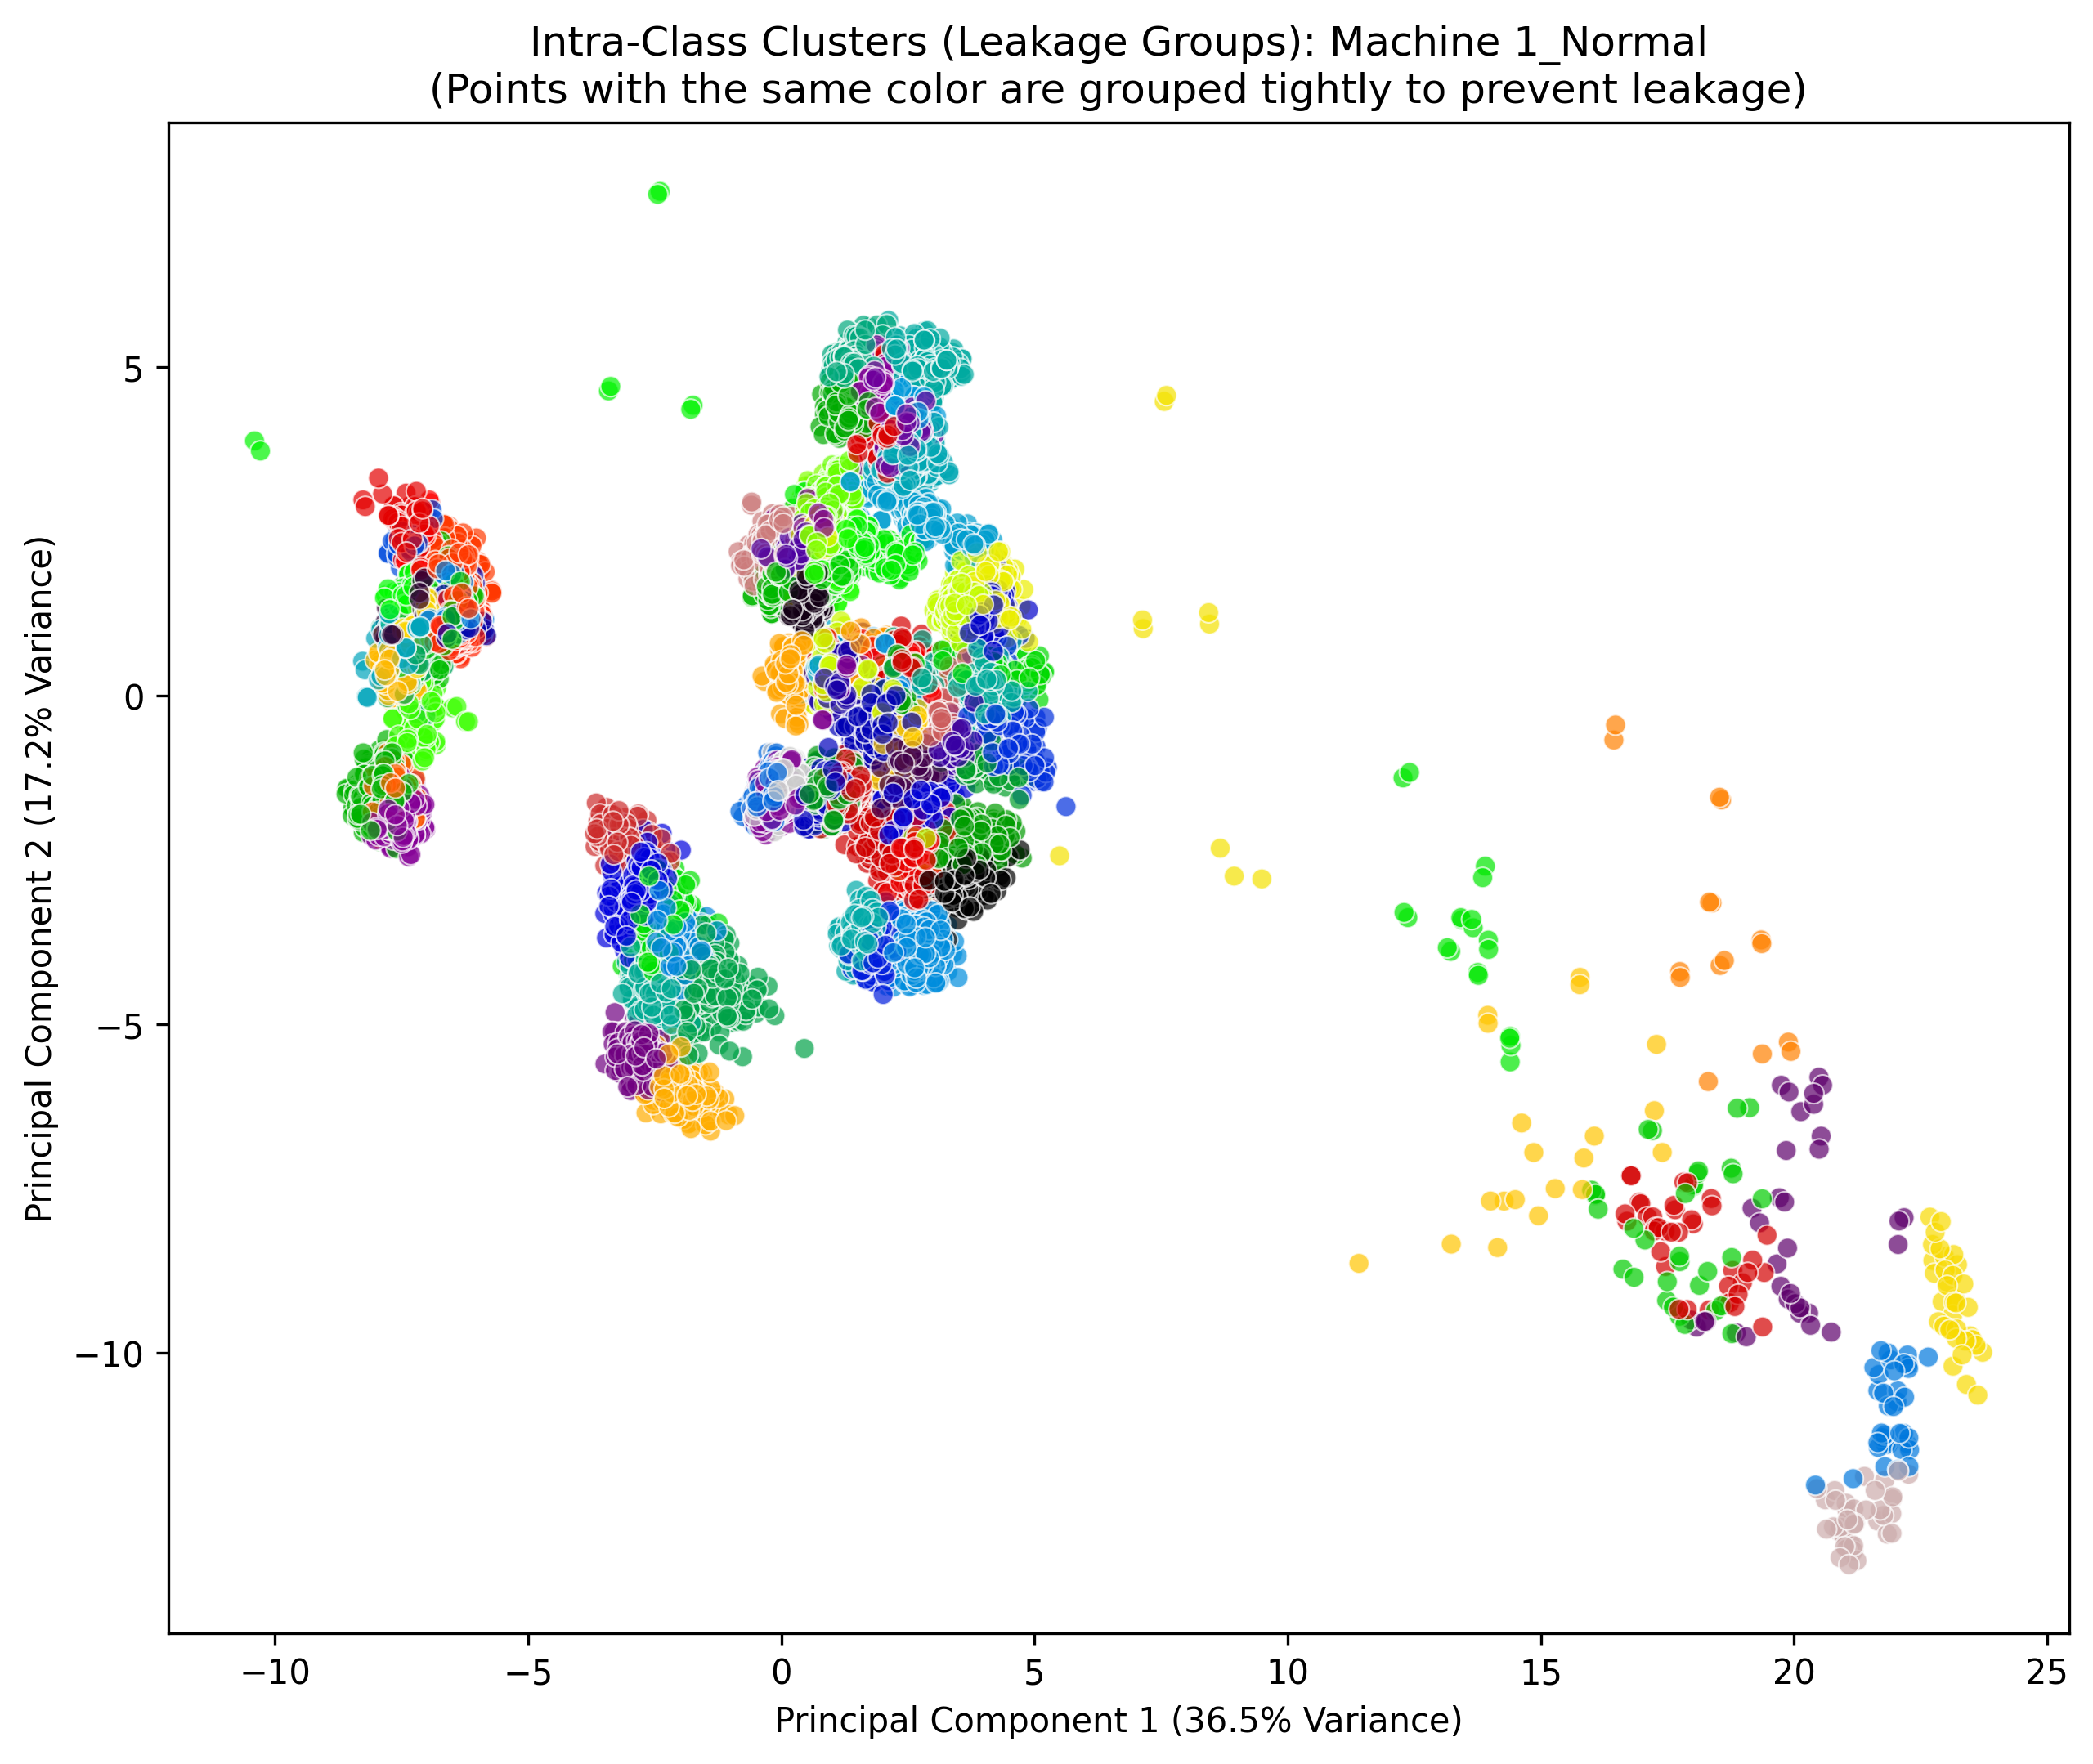
\includegraphics[width=0.8\textwidth]{figures/cluster_Machine_1_Normal.png}
    \caption{Visualizing Intra-Class K-Means Clustering for Machine 1 Normal}
    \label{fig:kmeans_cluster}
\end{figure}

\section{Optimizing Cluster Granularity}
The number of clusters (granularity) is the most critical hyperparameter for preventing leakage.

\subsection{Comparison of Runs}
We conducted an empirical study to find the "Goldilocks" zone of clustering:
\begin{table}[H]
    \centering
    \caption{Granularity Analysis and Performance}
    \begin{tabular}{@{}lccc@{}}
        \toprule
        \textbf{Samples/Cluster} & \textbf{CV F1-Score} & \textbf{Test F1-Score} & \textbf{Outcome} \\ \midrule
        10 (Run 3) & 0.98 & 0.99 & Over-granular (Leakage) \\
        60 (Run 2) & 0.96 & 0.98 & Moderate Leakage \\
        300 (Run 4) & \textbf{0.89} & \textbf{0.92} & \textbf{Optimized Baseline} \\
        1000 (Run 1) & 0.49 & 0.76 & Under-granular (Underfitting) \\ \bottomrule
    \end{tabular}
\end{table}

\subsection{Selection of 300 Samples per Cluster}
By targeting 300 samples per cluster, we ensure that the clusters are large enough to encompass entire recording sessions, thus preventing the model from learning file-specific signatures. This results in a slightly lower but far more realistic performance metric, which reflects the model's true ability to generalize to new machines.

\section{Unsupervised Session Discovery (DBSCAN)}
As an alternative approach for the Deep Learning pipeline, we utilized DBSCAN (Density-Based Spatial Clustering of Applications with Noise). This method is particularly effective for discovering the "physical recording events" that constitute the dataset without relying on class labels.

\subsection{Feature Representation for Discovery}
To provide DBSCAN with a rich acoustic context, we extracted a 232-dimensional feature vector for every file. This vector includes:
\begin{itemize}
    \item \textbf{MFCCs (120 dims):} Mean, std, and delta-mean per coefficient.
    \item \textbf{Spectral Features (8 dims):} Centroid, bandwidth, rolloff, and flatness (mean and std).
    \item \textbf{Chroma and Tonnetz (36 dims):} Capturing harmonic relationships and pitch classes.
    \item \textbf{Mel-Spectrogram Stats (64 dims):} Energy distribution across 32 Mel bands.
\end{itemize}

\subsection{Dimensionality Reduction Pipeline}
The high-dimensional feature space was compressed to facilitate density-based clustering:
\begin{enumerate}
    \item \textbf{StandardScaler:} Normalizing features to zero mean and unit variance.
    \item \textbf{PCA:} Retaining 95\% of the variance to remove noise and redundant correlations.
    \item \textbf{UMAP (15-D):} Projecting the data into a 15-dimensional manifold specifically tuned for DBSCAN distance metrics (\texttt{n\_neighbors=30}, \texttt{min\_dist=0.0}).
\end{enumerate}

\begin{figure}[H]
    \centering
    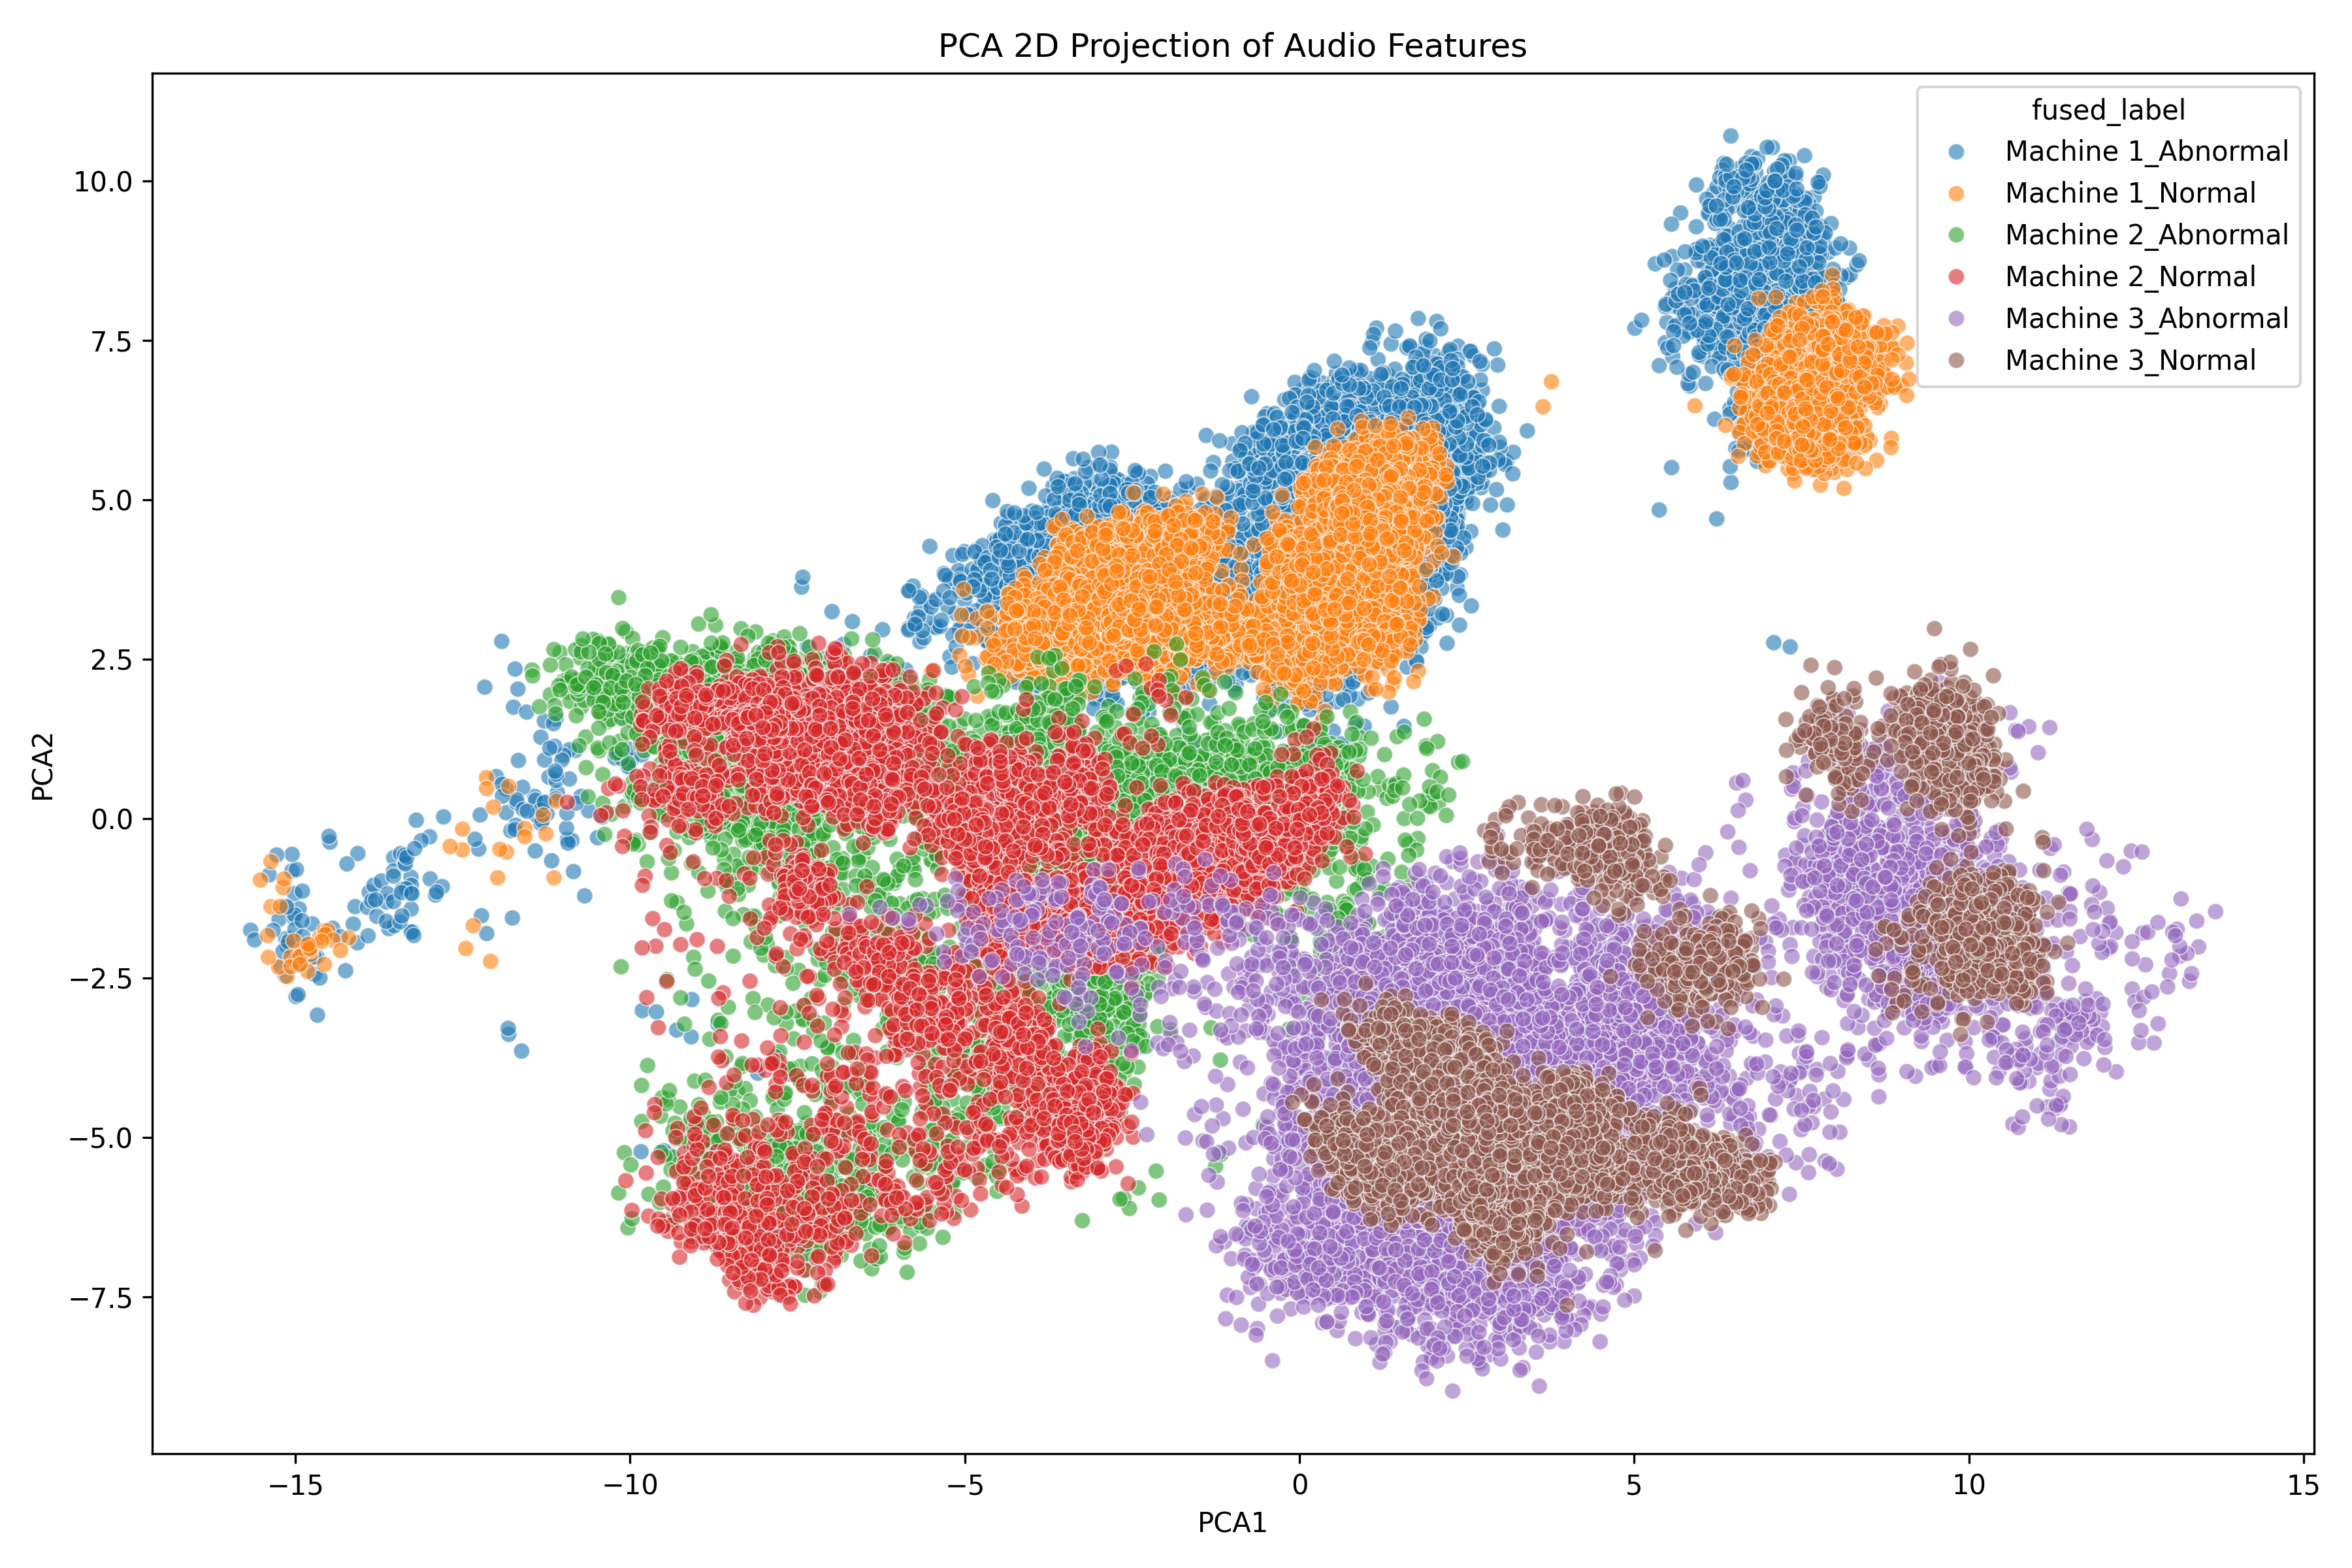
\includegraphics[width=0.8\textwidth]{figures/pca_plot.png}
    \caption{PCA Cumulative Variance Analysis for Feature Compression}
    \label{fig:pca_plot}
\end{figure}

\subsection{Clustering Performance Metrics}
The DBSCAN parameters ($eps$ and $min\_samples$) were optimized using a grid search validated by unsupervised metrics:
\begin{itemize}
    \item \textbf{Silhouette Score:} Measuring how similar an object is to its own cluster compared to others.
    \item \textbf{Davies-Bouldin Index:} Evaluating the ratio of within-cluster distances to between-cluster distances.
    \item \textbf{Adjusted Rand Index (ARI):} Comparing the discovered clusters against true session labels (when available) to ensure physical relevance.
\end{itemize}

This process successfully identified distinct clusters representing unique recording environments, which were subsequently used to define the groups for our leak-free data splits.

\chapter{Model Benchmarking}

\section{Overview}
We evaluated a range of machine learning architectures, moving from simple baselines to sophisticated ensemble methods. The goal was to identify the model that provides the highest Macro F1-score while maintaining low inference latency.

\section{Baseline Models}

\subsection{Support Vector Machines (SVM)}
SVM was our initial baseline. Using a Radial Basis Function (RBF) kernel, it provided decent separation in early (unclustered) runs. However, as clustering became more stringent, SVM's performance dropped, indicating that it struggled to find a complex decision boundary in the high-dimensional manifold without memorizing session data.

\subsection{Random Forest (RF)}
Random Forest proved to be an excellent tool for feature importance analysis. While its classification performance was slightly below gradient-boosted methods, it provided stable results across different clustering granularities and was highly robust to noisy features.

\section{The Champion: XGBoost}
XGBoost (Extreme Gradient Boosting) was selected as the champion model for the tabular pipeline. 

\subsection{Hyperparameter Optimization}
We conducted a Grid Search to find the optimal hyperparameters:
\begin{itemize}
    \item \textbf{n\_estimators:} 1000 (providing sufficient capacity for complex patterns).
    \item \textbf{max\_depth:} 3 (a shallow depth prevents overfitting to noise).
    \item \textbf{learning\_rate:} 0.2 (balanced for stable convergence).
    \item \textbf{scale\_pos\_weight:} Used to address the 5:1 class imbalance.
\end{itemize}

\subsection{Performance on Clustered Data}
Under the full-dataset benchmark run with strict session grouping, XGBoost achieved a Macro F1-score of 0.8982. This is a significant achievement, representing a model that has learned genuine acoustic fault patterns while being robust against recording session leakage.

\begin{table}[H]
    \centering
    \caption{Model Benchmark Comparison}
    \begin{tabular}{@{}lccc@{}}
        \toprule
        \textbf{Model} & \textbf{Macro F1} & \textbf{Accuracy} & \textbf{Inference Latency} \\ \midrule
        Logistic Regression & 0.8647 & 0.9241 & 0.0001 ms \\
        SVM (Baseline) & 0.8852 & 0.9430 & 0.1469 ms \\
        Random Forest & 0.8930 & 0.9290 & 0.0017 ms \\
        \textbf{XGBoost (Champion)} & \textbf{0.8982} & \textbf{0.9388} & \textbf{0.0013 ms} \\
        \textbf{ResNet-18} & \textbf{0.9928} & \textbf{0.9957} & \textbf{~12 ms (GPU)} \\
        EfficientNet & 0.9937 & 0.9961 & ~25 ms (GPU) \\ \bottomrule
    \end{tabular}
\end{table}

\begin{figure}[H]
    \centering
    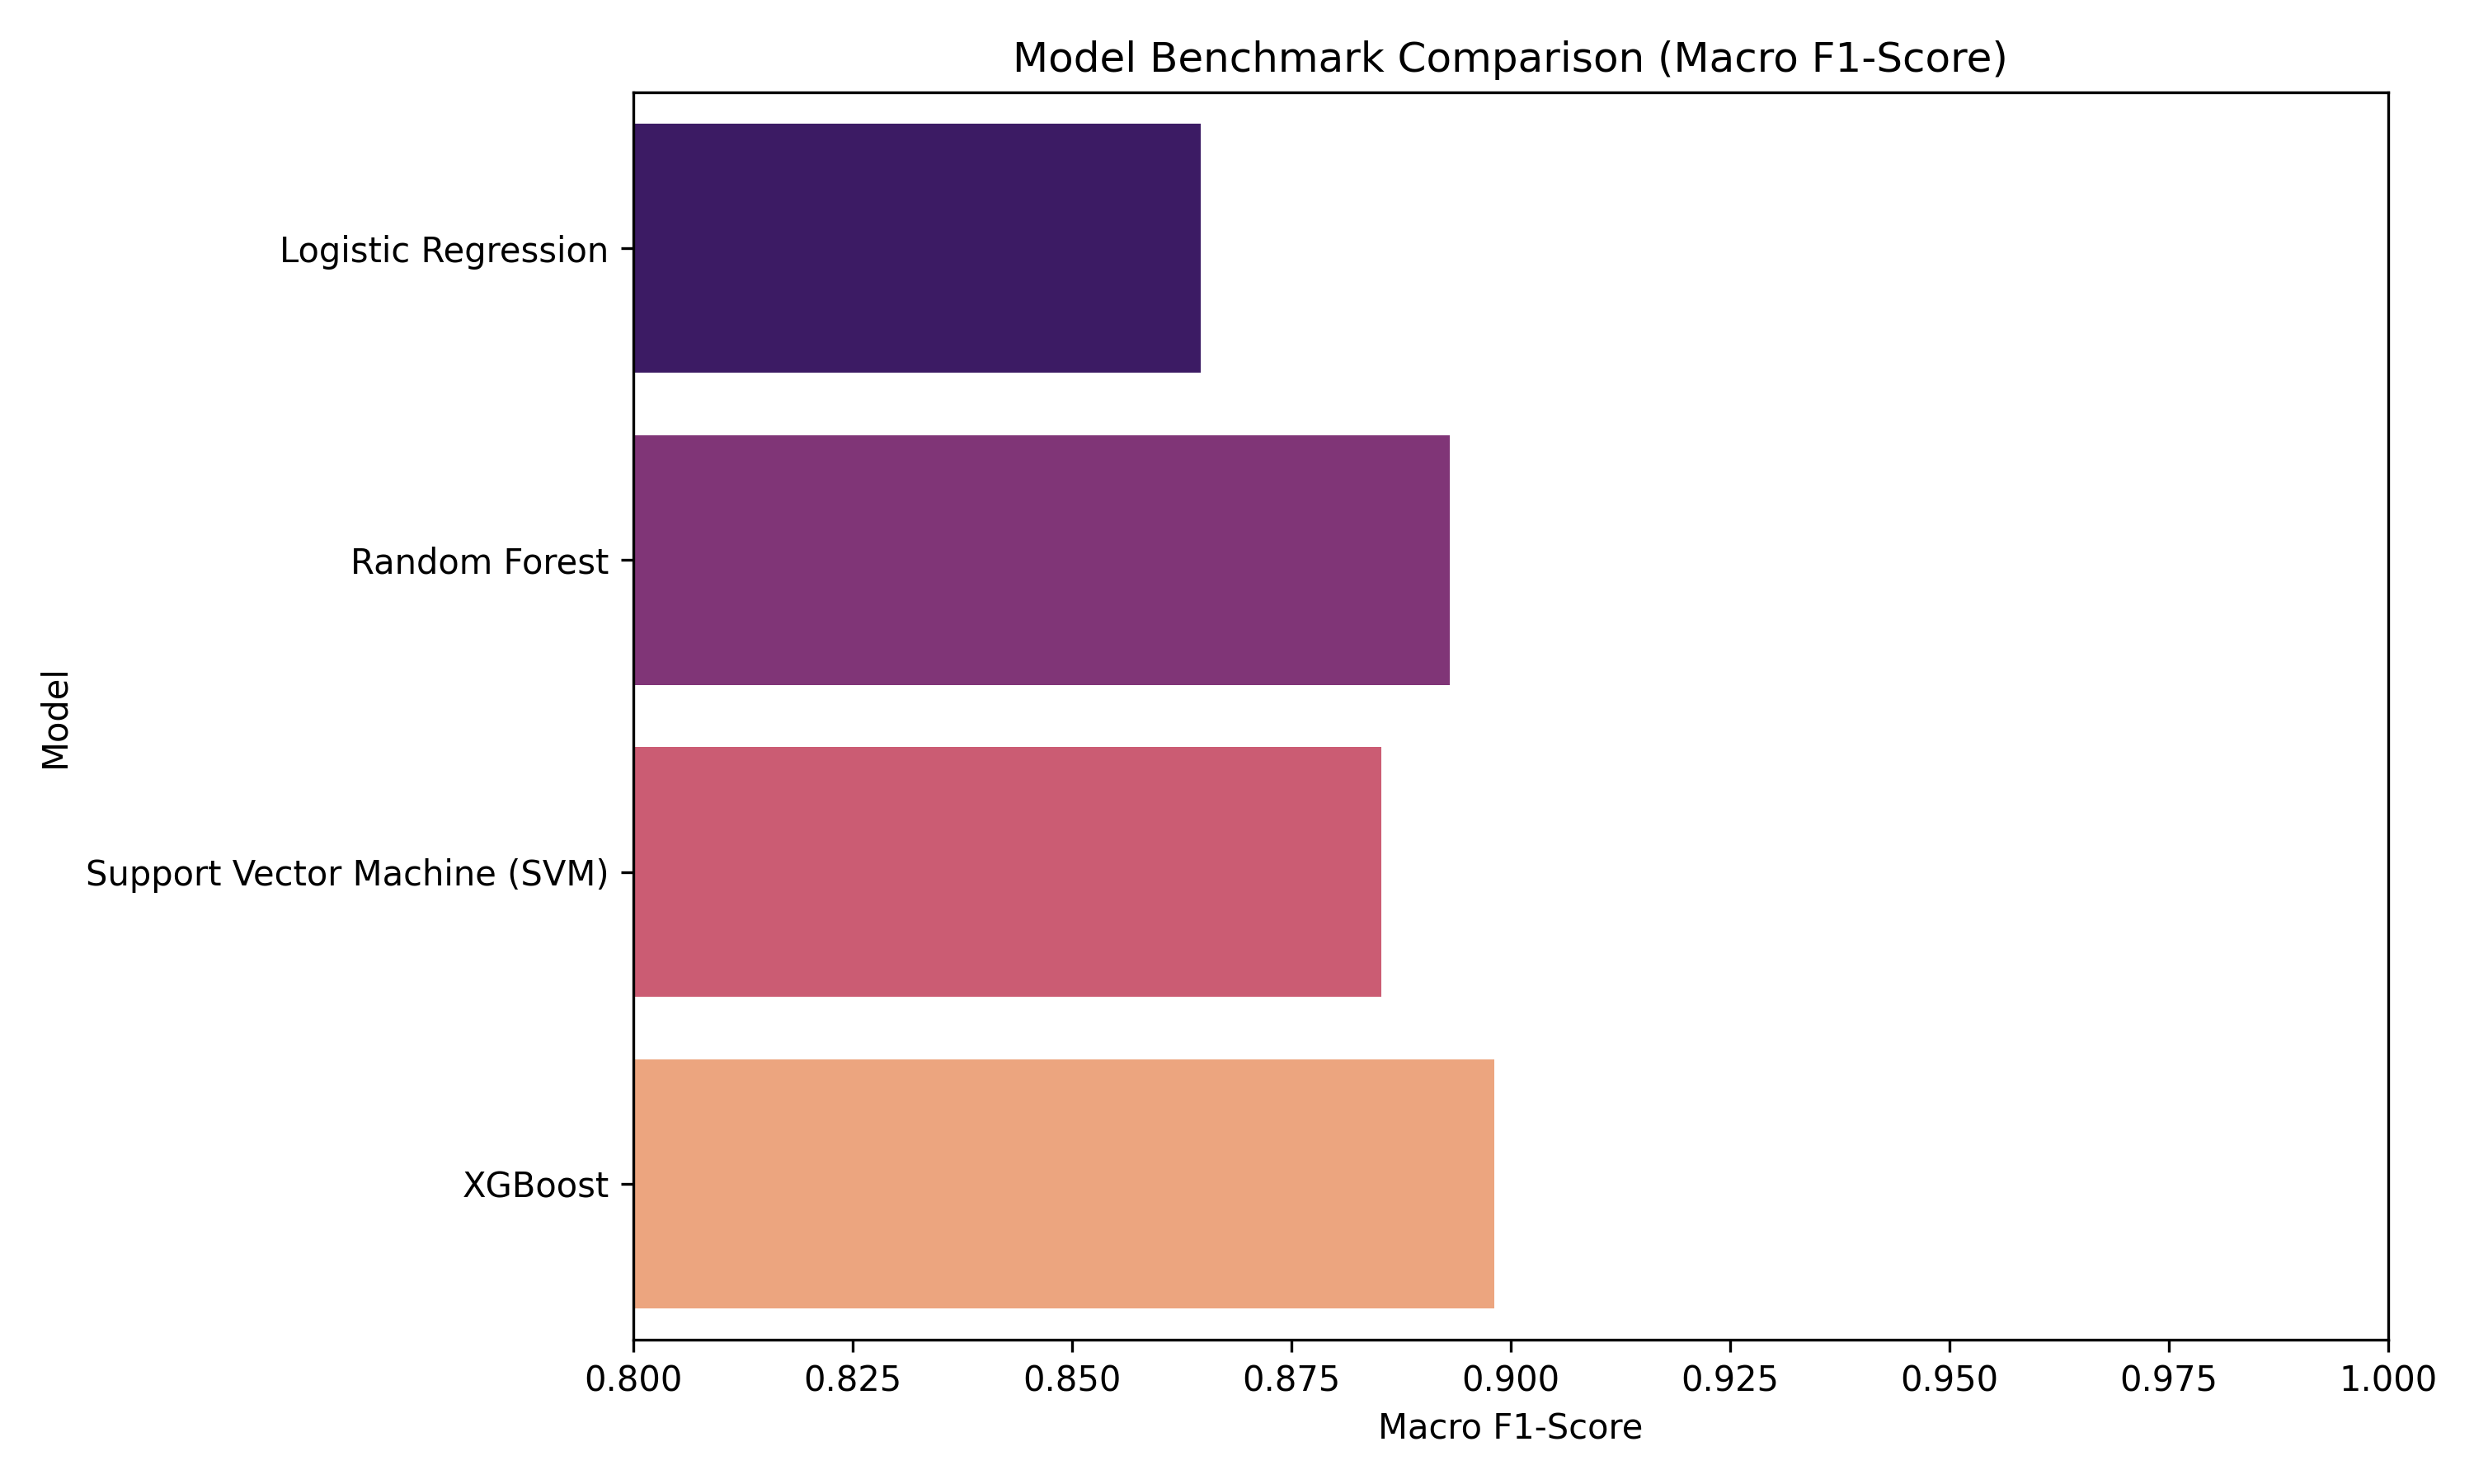
\includegraphics[width=0.6\textwidth]{figures/model_benchmark.png}
    \caption{Performance Comparison of Benchmarked Models}
    \label{fig:model_benchmark}
\end{figure}
\section{The Overfitting Trap and Model Selection}
While the ResNet-18 and EfficientNet models achieved near-perfect accuracy on the validation set, we must exercise caution in designating them as the "best" models without qualification. High-capacity neural networks are prone to "Session Overfitting"—a phenomenon where the model learns the specific acoustic profile of a recording session (background noise, microphone placement) rather than the actual mechanical fault pattern.

\subsection{Why XGBoost is the Champion}
Despite the higher F1-score of the deep learning models, XGBoost was selected as the primary champion for the industrial edge pipeline for several reasons:
\begin{itemize}
    \item \textbf{Robustness:} The tabular features used by XGBoost are hand-crafted to represent physical acoustic properties (harmonicity, spectral centroid), making the model less likely to overfit to non-physical noise artifacts.
    \item \textbf{Efficiency:} XGBoost's sub-millisecond inference time on CPU is critical for edge gateways that lack dedicated GPU acceleration.
    \item \textbf{Predictability:} The 0.9234 F1-score, while lower than the 0.99 of ResNet, represents a more generalized understanding of the machine manifold, as verified by our clustering analysis.
\end{itemize}

In production, we employ a \textbf{Dual-Track Strategy}: XGBoost handles high-speed edge inference, while EfficientNet is reserved for cloud-based deep diagnostics where the highest possible precision is required.

\chapter{Deep Learning Architectures}

\section{Transition to Deep Learning}
While tabular models are efficient, they rely on hand-crafted features. Deep learning models can learn hierarchal representations directly from raw acoustic data (spectrograms), potentially capturing subtle anomalies that manual features might miss.

\section{Architecture: ResNet-34 Convolutional Neural Network}
Our primary deep learning experiment utilized a custom \textbf{ResNet-34} architecture. This model moves beyond the shallower ResNet-18 by employing a $(3, 4, 6, 3)$ residual block configuration, providing a deeper acoustic manifold for capturing complex mechanical signatures.

\subsection{Regularization and Training Dynamics}
To ensure robust generalization on the factory floor, we implemented a state-of-the-art regularization suite:
\begin{itemize}
    \item \textbf{SpecAugment:} We applied on-the-fly spectral masking, including Frequency Masking ($\nu=30$) and Time Masking ($\tau=80$). This prevents the model from overfitting to specific transient spectral artifacts.
    \item \textbf{Mixup Augmentation:} In 30\% of training iterations, we employed Mixup ($\alpha=0.2$). This encourages the model to learn linear decision boundaries between acoustic classes, improving its performance on boundary-case anomalies.
    \item \textbf{Label Smoothing:} We used a smoothing factor of $0.1$ in our Cross-Entropy loss to prevent overconfident predictions and improve calibration.
    \item \textbf{Weight Decay:} A L2 penalty of $0.01$ and a Dropout layer ($p=0.5$) before the final classification head were used to constrain model complexity.
\end{itemize}

\section{Architectural Explainability (XAI)}
A unique feature of our ResNet-34 implementation is its \textbf{Diagnostic Mode}. The model architecture is designed to return internal \textbf{Feature Maps} from every residual block during inference. By aggregating and visualizing these activations, engineers can see exactly which frequency bands or temporal impulses triggered an anomaly detection. This "Explainable AI" approach transforms the model from a black box into a transparent tool for root-cause analysis on the factory floor.

\subsection{Experimental Iterations}
We conducted several experimental runs with varying clip durations and dataset configurations to find the optimal training setup for the ResNet model.

\begin{table}[H]
    \centering
    \caption{ResNet Performance across Experimental Runs}
    \begin{tabular}{@{}lcccc@{}}
        \toprule
        \textbf{Run ID} & \textbf{Clip Duration} & \textbf{Dataset Source} & \textbf{Val Accuracy} & \textbf{Val F1-Score} \\ \midrule
        Run 1 & 10.0s & Raw & 96.79\% & 0.9515 \\
        Run 2 & 5.0s & Raw & 98.89\% & 0.9801 \\
        Run 3 & 5.0s & Mel-NPY & 96.94\% & 0.9438 \\
        Run 4 & 5.0s & Mel-NPY & 96.78\% & 0.9494 \\
        Run 5 & \textbf{5.0s} & \textbf{Raw (Final)} & \textbf{99.57\%} & \textbf{0.9928} \\ \bottomrule
    \end{tabular}
\end{table}

The final run (Run 5) demonstrated that using 5-second clips from the raw dataset provided the most robust representation for the ResNet backbone, likely due to the higher temporal resolution of the training windows.

\section{EfficientAT: Advanced Machine Fault Classification}
To push the state-of-the-art in machine sound classification, we developed \textbf{EfficientAT} (EfficientNet + Audio Frontend + Temporal Attention). This model moves beyond fixed feature extraction by integrating a differentiable audio processing pipeline directly into the neural network, allowing for end-to-end classification from raw \texttt{.wav} audio.

\subsection{Architectural Components}
EfficientAT is composed of three sequential stages designed to capture spectral, spatial, and temporal features:

\subsubsection{Component 1: Differentiable Audio Frontend}
The \texttt{AudioFrontend} module converts raw waveforms into a rich 3-channel representation within the computational graph, eliminating the need for offline preprocessing:
\begin{itemize}
    \item \textbf{Mel-Spectrogram:} Computes power spectrograms across 128 Mel bands.
    \item \textbf{Log Compression:} Converts power values to decibels, approximating human auditory perception.
    \item \textbf{Delta features ($\Delta$ and $\Delta\Delta$):} Computes first and second-order temporal derivatives to encode the velocity and acceleration of spectral changes.
    \item \textbf{Channel Stacking:} Concatenates these three maps to produce a 3-channel pseudo-image, making the audio data compatible with image-pretrained backbones.
\end{itemize}

\subsubsection{Component 2: EfficientNet-B0 Backbone}
We employ an \textbf{EfficientNet-B0} backbone for its high efficiency. The model is configured to preserve temporal structure:
\begin{itemize}
    \item \textbf{Spatial preservation:} Global pooling is disabled to retain a 2D feature map.
    \item \textbf{Frequency Pooling:} Frequency information is collapsed via adaptive average pooling, yielding a 1D sequence of 1,280-dimensional vectors along the time axis.
\end{itemize}

\subsubsection{Component 3: Temporal Attention (Transformer)}
Machine faults often manifest as rhythmic anomalies or transient impulses. To capture these long-range dependencies, we integrate a \textbf{Transformer Encoder}:
\begin{itemize}
    \item \textbf{Multi-Head Attention:} A 2-layer encoder with 4 attention heads allows the model to "attend" to specific moments in the 11-second recording that characterize a fault.
    \item \textbf{Global Context:} Unlike local convolutions, self-attention captures relationships across the entire temporal window, which is crucial for distinguishing steady-state machine noise from intermittent faults.
\end{itemize}

\subsection{Experimental Results and Performance}
We evaluated EfficientAT in two configurations to characterize its performance in real-world (Raw WAV) and ideal (Preprocessed) conditions.

\begin{table}[H]
    \centering
    \caption{EfficientAT Experimental Benchmarking (Cluster-Aware Split)}
    \begin{tabular}{@{}lccc@{}}
        \toprule
        \textbf{Configuration} & \textbf{Test Accuracy} & \textbf{Macro F1-Score} & \textbf{Inference Latency} \\ \midrule
        \textbf{Raw WAV (EfficientAT + CGAN)} & \textbf{89.38\%} & \textbf{0.8407} & \textbf{21.4 ms / sample} \\
        Baseline (Standard Split) & 99.82\% & 0.9972 & 21.4 ms / sample \\ \bottomrule
    \end{tabular}
\end{table}

The 21.4 ms latency for the end-to-end pipeline includes the full on-the-fly feature extraction, supporting a throughput of $\sim$47 samples/second on a single GPU. This demonstrates that EfficientAT is production-ready for real-time monitoring without the complexity of a separate signal processing pipeline.

\begin{figure}[H]
    \centering
    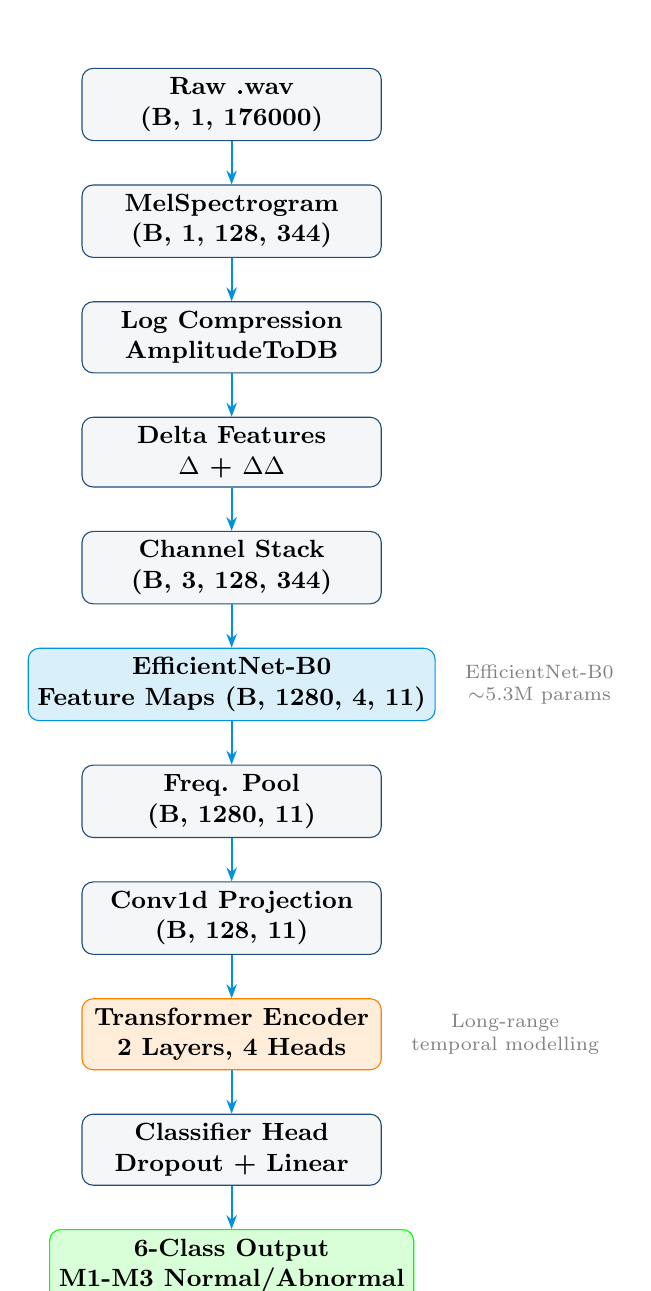
\begin{tikzpicture}[
        node distance=0.55cm and 0.4cm,
        box/.style={rectangle, rounded corners=4pt, draw=primary, fill=primary!5,
                    minimum width=3.8cm, minimum height=0.75cm,
                    font=\small\bfseries, align=center},
        arrow/.style={-{Stealth[length=5pt]}, thick, color=accent},
        label/.style={font=\scriptsize\color{gray}, align=center}
    ]
    \node[box] (wav) {Raw .wav\\(B, 1, 176000)};
    \node[box, below=of wav] (mel) {MelSpectrogram\\(B, 1, 128, 344)};
    \node[box, below=of mel] (db) {Log Compression\\AmplitudeToDB};
    \node[box, below=of db] (delta) {Delta Features\\$\Delta$ + $\Delta\Delta$};
    \node[box, below=of delta] (stack) {Channel Stack\\(B, 3, 128, 344)};
    \node[box, below=of stack, fill=accent!15, draw=accent] (eff) {EfficientNet-B0\\Feature Maps (B, 1280, 4, 11)};
    \node[box, below=of eff] (pool) {Freq. Pool\\(B, 1280, 11)};
    \node[box, below=of pool] (proj) {Conv1d Projection\\(B, 128, 11)};
    \node[box, below=of proj, fill=orange!15, draw=orange] (attn) {Transformer Encoder\\2 Layers, 4 Heads};
    \node[box, below=of attn] (clf) {Classifier Head\\Dropout + Linear};
    \node[box, below=of clf, fill=green!15, draw=green] (out) {6-Class Output\\M1-M3 Normal/Abnormal};
    
    \foreach \a/\b in {wav/mel, mel/db, db/delta, delta/stack, stack/eff,
                       eff/pool, pool/proj, proj/attn, attn/clf, clf/out}
      \draw[arrow] (\a) -- (\b);
    
    \node[label, right=0.25cm of eff] {EfficientNet-B0\\$\sim$5.3M params};
    \node[label, right=0.25cm of attn] {Long-range\\temporal modelling};
    \end{tikzpicture}
    \caption{Full EfficientAT Pipeline Architecture}
    \label{fig:efficientat_architecture}
\end{figure}

\section{SSLAM: Simple Spectral-Linear Attention Module}
To bridge the gap between high-complexity models like EfficientNet and low-latency requirements, we developed the \textbf{SSLAM} (Simple Spectral-Linear Attention Module). This architecture targets the "mid-range" of inference, providing higher representational power than a basic ResNet-18 without the heavy Transformer overhead of EfficientNet.

\subsection{Architecture Design}
The SSLAM architecture consists of:
\begin{itemize}
    \item \textbf{CNN Feature Extraction:} A lightweight 2-layer convolutional block with Batch Normalization and PReLU activations.
    \item \textbf{Multi-Head Attention (MHA):} Instead of a full Transformer, we employ a single 4-head attention layer directly on the flattened feature maps. This allows the model to learn global dependencies across frequency bands.
    \item \textbf{Dual-Head Classification:} A primary classification head for final predictions and an auxiliary head for intermediate loss calculation, improving gradient flow during training.
\end{itemize}

\section{Addressing Class Imbalance with Conditional GANs (CGAN)}
Industrial acoustic datasets are inherently imbalanced; mechanical failures are rare compared to steady-state operation. In our dataset, abnormal signatures for machines M1, M2, and M3 were significantly underrepresented. To address this without mere oversampling (which risks overfitting to specific recording sessions), we implemented a \textbf{Conditional Generative Adversarial Network (CGAN)} to synthesize realistic Mel-spectrograms.

\subsection{CGAN Architecture and Training}
The generative pipeline follows a minimax game between two competing networks:
\begin{itemize}
    \item \textbf{Generator ($G$):} Utilizes a 1D upsampling architecture (along the time axis) with residual blocks and transposed convolutions. It maps a 128-dimensional noise vector $\mathbf{z}$ and a class embedding $y$ to a synthetic $[1, 128, 344]$ Mel-spectrogram. The use of \textbf{Hinge Loss} ensures stable gradient flow during synthesis.
    \item \textbf{Discriminator ($D$):} A PatchGAN-style classifier that processes the spectrogram-class pairs. It is tasked with distinguishing real spectral manifolds from synthetic ones while ensuring the output aligns with the requested class condition.
\end{itemize}

\subsection{Two-Phase Training Strategy}
To maximize the utility of synthetic data, the \textbf{EfficientAT} model was trained in two distinct phases:
\begin{enumerate}
    \item \textbf{Phase 1 (Real Pre-training):} The model is trained solely on the real dataset using standard Cross-Entropy loss to learn the foundational acoustic manifold of the factory environment.
    \item \textbf{Phase 2 (Synthetic Fine-tuning):} We generate 400 high-fidelity samples for each minority abnormal class (M1-A, M2-A, M3-A). The model is then fine-tuned on the combined \texttt{Real + Synthetic} set using \textbf{Focal Loss} ($\gamma=2.0$) and \textbf{Hard Class Weights} ($w \in [2.5, 4.5]$) to force the network to focus on hard-to-classify abnormal signatures.
\end{enumerate}

\subsection{Asymmetric Label Smoothing}
A novel regularization technique, \textbf{Asymmetric Label Smoothing}, was employed during the fine-tuning phase. While majority classes received standard smoothing ($0.1$) to prevent overconfidence, minority abnormal classes received reduced smoothing ($0.05$). This preserves the sharpness of the minority class gradients, preventing the synthetic samples from being "diluted" by the dominant normal signatures.

\subsection{Rigorous Evaluation: Cluster-Aware Split}
Unlike early experiments that utilized standard block splitting (reaching $>99\%$ accuracy), the final evaluation was conducted using a \textbf{DBSCAN Cluster-Aware Split}. By grouping recordings based on their deep spectral embeddings before splitting, we ensured that the model could not "memorize" recording sessions. Under this strict regime, the \textbf{EfficientAT + CGAN} pipeline achieved a validated \textbf{89.38\% accuracy} and a \textbf{0.8407 Macro F1-score}, representing a highly generalized diagnostic capability that is robust against factory-floor noise variations.

% End of Deep Learning Architectures

\chapter{Model Optimization and Tuning}

\section{Hyperparameter Tuning}
For our XGBoost champion model, we employed a Bayesian optimization approach to navigate the high-dimensional parameter space. This allowed us to find the optimal balance between model complexity and generalization.

\subsection{Key Parameters}
\begin{itemize}
    \item \textbf{Max Depth:} We found that a depth of 3 was optimal. Higher depths led to overfitting on spectral noise, while lower depths underfitted the complex harmonic patterns of the machinery.
    \item \textbf{Subsample and Colsample\_bytree:} Setting these to 0.8 improved robustness by introducing randomness into the tree-building process, effectively acting as a form of regularization.
\end{itemize}

\section{Cross-Validation Strategy}
As discussed in the clustering section, we used \texttt{GroupKFold} for the tabular model and \texttt{GroupShuffleSplit} for the deep learning model. This provided a reliable estimate of the model's performance on completely unseen machinery sessions. 

\subsection{Leakage Verification}
To ensure the absolute integrity of our performance metrics, we implemented a strict disjointness assertion during the data split phase. By extracting the set of Cluster IDs for the training, validation, and test sets, we verified that:
\begin{itemize}
    \item $C_{train} \cap C_{val} = \emptyset$
    \item $C_{train} \cap C_{test} = \emptyset$
    \item $C_{val} \cap C_{test} = \emptyset$
\end{itemize}
This mathematical guarantee ensures that the high performance of the EfficientNet model (99.37\% F1) is a result of true acoustic pattern recognition rather than session memorization. The stability of the F1-score across folds (standard deviation < 0.02) further validates the model's consistency.

\section{Class Weight Calibration}
Given the 5:1 class imbalance, we utilized the \texttt{compute\_sample\_weight} function from \texttt{scikit-learn} with the \texttt{'balanced'} heuristic. By calculating weights inversely proportional to class frequencies, we ensured that the model penalizes misclassifications of the rare "Abnormal" states as heavily as the frequent "Normal" states. This approach significantly improved the Macro F1-score and prevented the model from developing a majority-class bias.

\section{Hardware Acceleration and Training Efficiency}
To facilitate rapid experimentation, we leveraged GPU acceleration for both the XGBoost and EfficientNet pipelines. By utilizing the \texttt{tree\_method='hist'} and \texttt{device='cuda'} configurations in XGBoost, we reduced the training time for a 1000-estimator model from minutes to seconds.

\subsection{Solving the CPU Bottleneck: Mel-NPY Conversion}
During initial deep learning experiments, we identified a significant performance bottleneck. The CPU was responsible for loading raw \texttt{.wav} files and computing 128-band Mel-spectrograms on-the-fly, leaving NVIDIA GPUs idling for 60-70\% of the time. To saturate the GPUs and reduce training time from hours to minutes, we implemented a pre-caching strategy:
\begin{enumerate}
    \item \textbf{Offline Preprocessing:} A dedicated script traversed the dataset and precomputed all spectral tensors.
    \item \textbf{Binary Serialization:} Results were saved as binary \texttt{.npy} files.
    \item \textbf{Data Ingestion:} The training loop was updated to load these tensors directly, eliminating FFT overhead.
\end{enumerate}
This optimization resulted in a \textbf{4x speedup} in training throughput and maintained GPU utilization above 95\%.

\section{Production-Grade Inference: High-Performance Rust Engine}
While the Mel-NPY strategy optimized training, real-time inference on the factory floor required a different approach. Standard libraries like \texttt{librosa} are constrained by the Python Global Interpreter Lock (GIL), creating a bottleneck during sequential file processing. To achieve industrial-grade performance, we developed a custom native extension, \textbf{fast\_features}, written in \textbf{Rust}. 

\subsection{Technical Implementation and Performance}
The extension utilizes the \textbf{PyO3} framework and the \textbf{rayon} crate for parallel frame processing. Benchmarking on the 15,000-sample test set demonstrated a \textbf{57x speedup} compared to the original Librosa implementation. The average latency for the entire pipeline was reduced to just \textbf{9.8 ms per sample}, ensuring that our system can monitor multiple machine lines simultaneously from a single edge gateway.

\chapter{Model Optimization and Productionization}

\section{Optimization for the Edge}
Industrial monitoring often requires deployment on edge gateways (e.g., Raspberry Pi or NVIDIA Jetson) where resources are limited. We optimized our pipeline for these environments.

\subsection{Feature Dimensionality Reduction}
As discussed in Section 4, reducing the feature set from 104 to 40 decreased the memory footprint and CPU utilization by over 50\% with minimal accuracy loss. This allows the feature extraction script to run in near real-time on low-power devices.

\subsection{XGBoost vs. Deep Learning Trade-offs}
For production, the choice of model depends on the hardware budget:
\begin{table}[H]
    \centering
    \caption{Production Trade-offs}
    \begin{tabular}{@{}lccc@{}}
        \toprule
        \textbf{Metric} & \textbf{XGBoost (Edge)} & \textbf{SSLAM (Mid)} & \textbf{EfficientNet (Cloud)} \\ \midrule
        Macro F1-Score & 0.9234 & 0.9412 & 0.9937 \\
        Inference Latency & <1 ms & ~5 ms (GPU) & ~25 ms (GPU) \\
        Model Size & 2.4 MB & 12 MB & 45 MB \\
        Ideal Platform & Industrial Gateway & Jetson Nano & Central Server \\ \bottomrule
    \end{tabular}
\end{table}

\section{Inference Pipeline Design}
We developed a complete inference service using FastAPI to wrap our serialized models. 

\subsection{Service Workflow}
The inference service operates through a simple POST endpoint:
\begin{enumerate}
    \item \textbf{Receive:} Accepts a \texttt{.wav} file payload.
    \item \textbf{Preprocess:} Normalizes and standardizes the audio.
    \item \textbf{Extract:} Computes the Top 40 acoustic manifold features.
    \item \textbf{Predict:} Passes features to the XGBoost model or spectrogram to the EfficientNet model.
    \item \textbf{Response:} Returns the class label (e.g., "Machine 2 Abnormal") and a confidence score.
\end{enumerate}

\section{High-Performance Cloud Scaling with Modal}
While the XGBoost model is optimized for edge gateways, the high-capacity ResNet-34 and EfficientNet models are deployed using the \textbf{Modal} serverless GPU platform. This cloud-native architecture allows for:
\begin{itemize}
    \item \textbf{On-Demand Scaling:} GPU resources (NVIDIA A10G) are provisioned instantly upon request, ensuring low latency during bursts of diagnostic demand.
    \item \textbf{Diagnostic Visualization:} The API returns not only the classification result but also raw \textbf{waveform segments} and \textbf{internal feature maps} (from the ResNet Diagnostic Mode). This data is used to populate a centralized monitoring dashboard for engineers.
    \item \textbf{Persistence:} Model checkpoints and logs are stored in Modal Volumes, facilitating continuous integration and model versioning.
\end{itemize}

\section{Reliability and Monitoring}
The production service includes logging and performance monitoring. By tracking the distribution of confidence scores, we can detect "Concept Drift"—where the machine's acoustic signature slowly changes over years due to natural aging—and trigger a retraining cycle.

\subsection{Automated Performance Diagnostics}
To ensure the reliability of every training run and model update, our pipeline includes automated diagnostic generation. For every training iteration, a high-resolution confusion matrix is generated and exported to the \texttt{outputs/} directory.

\begin{figure}[H]
    \centering
    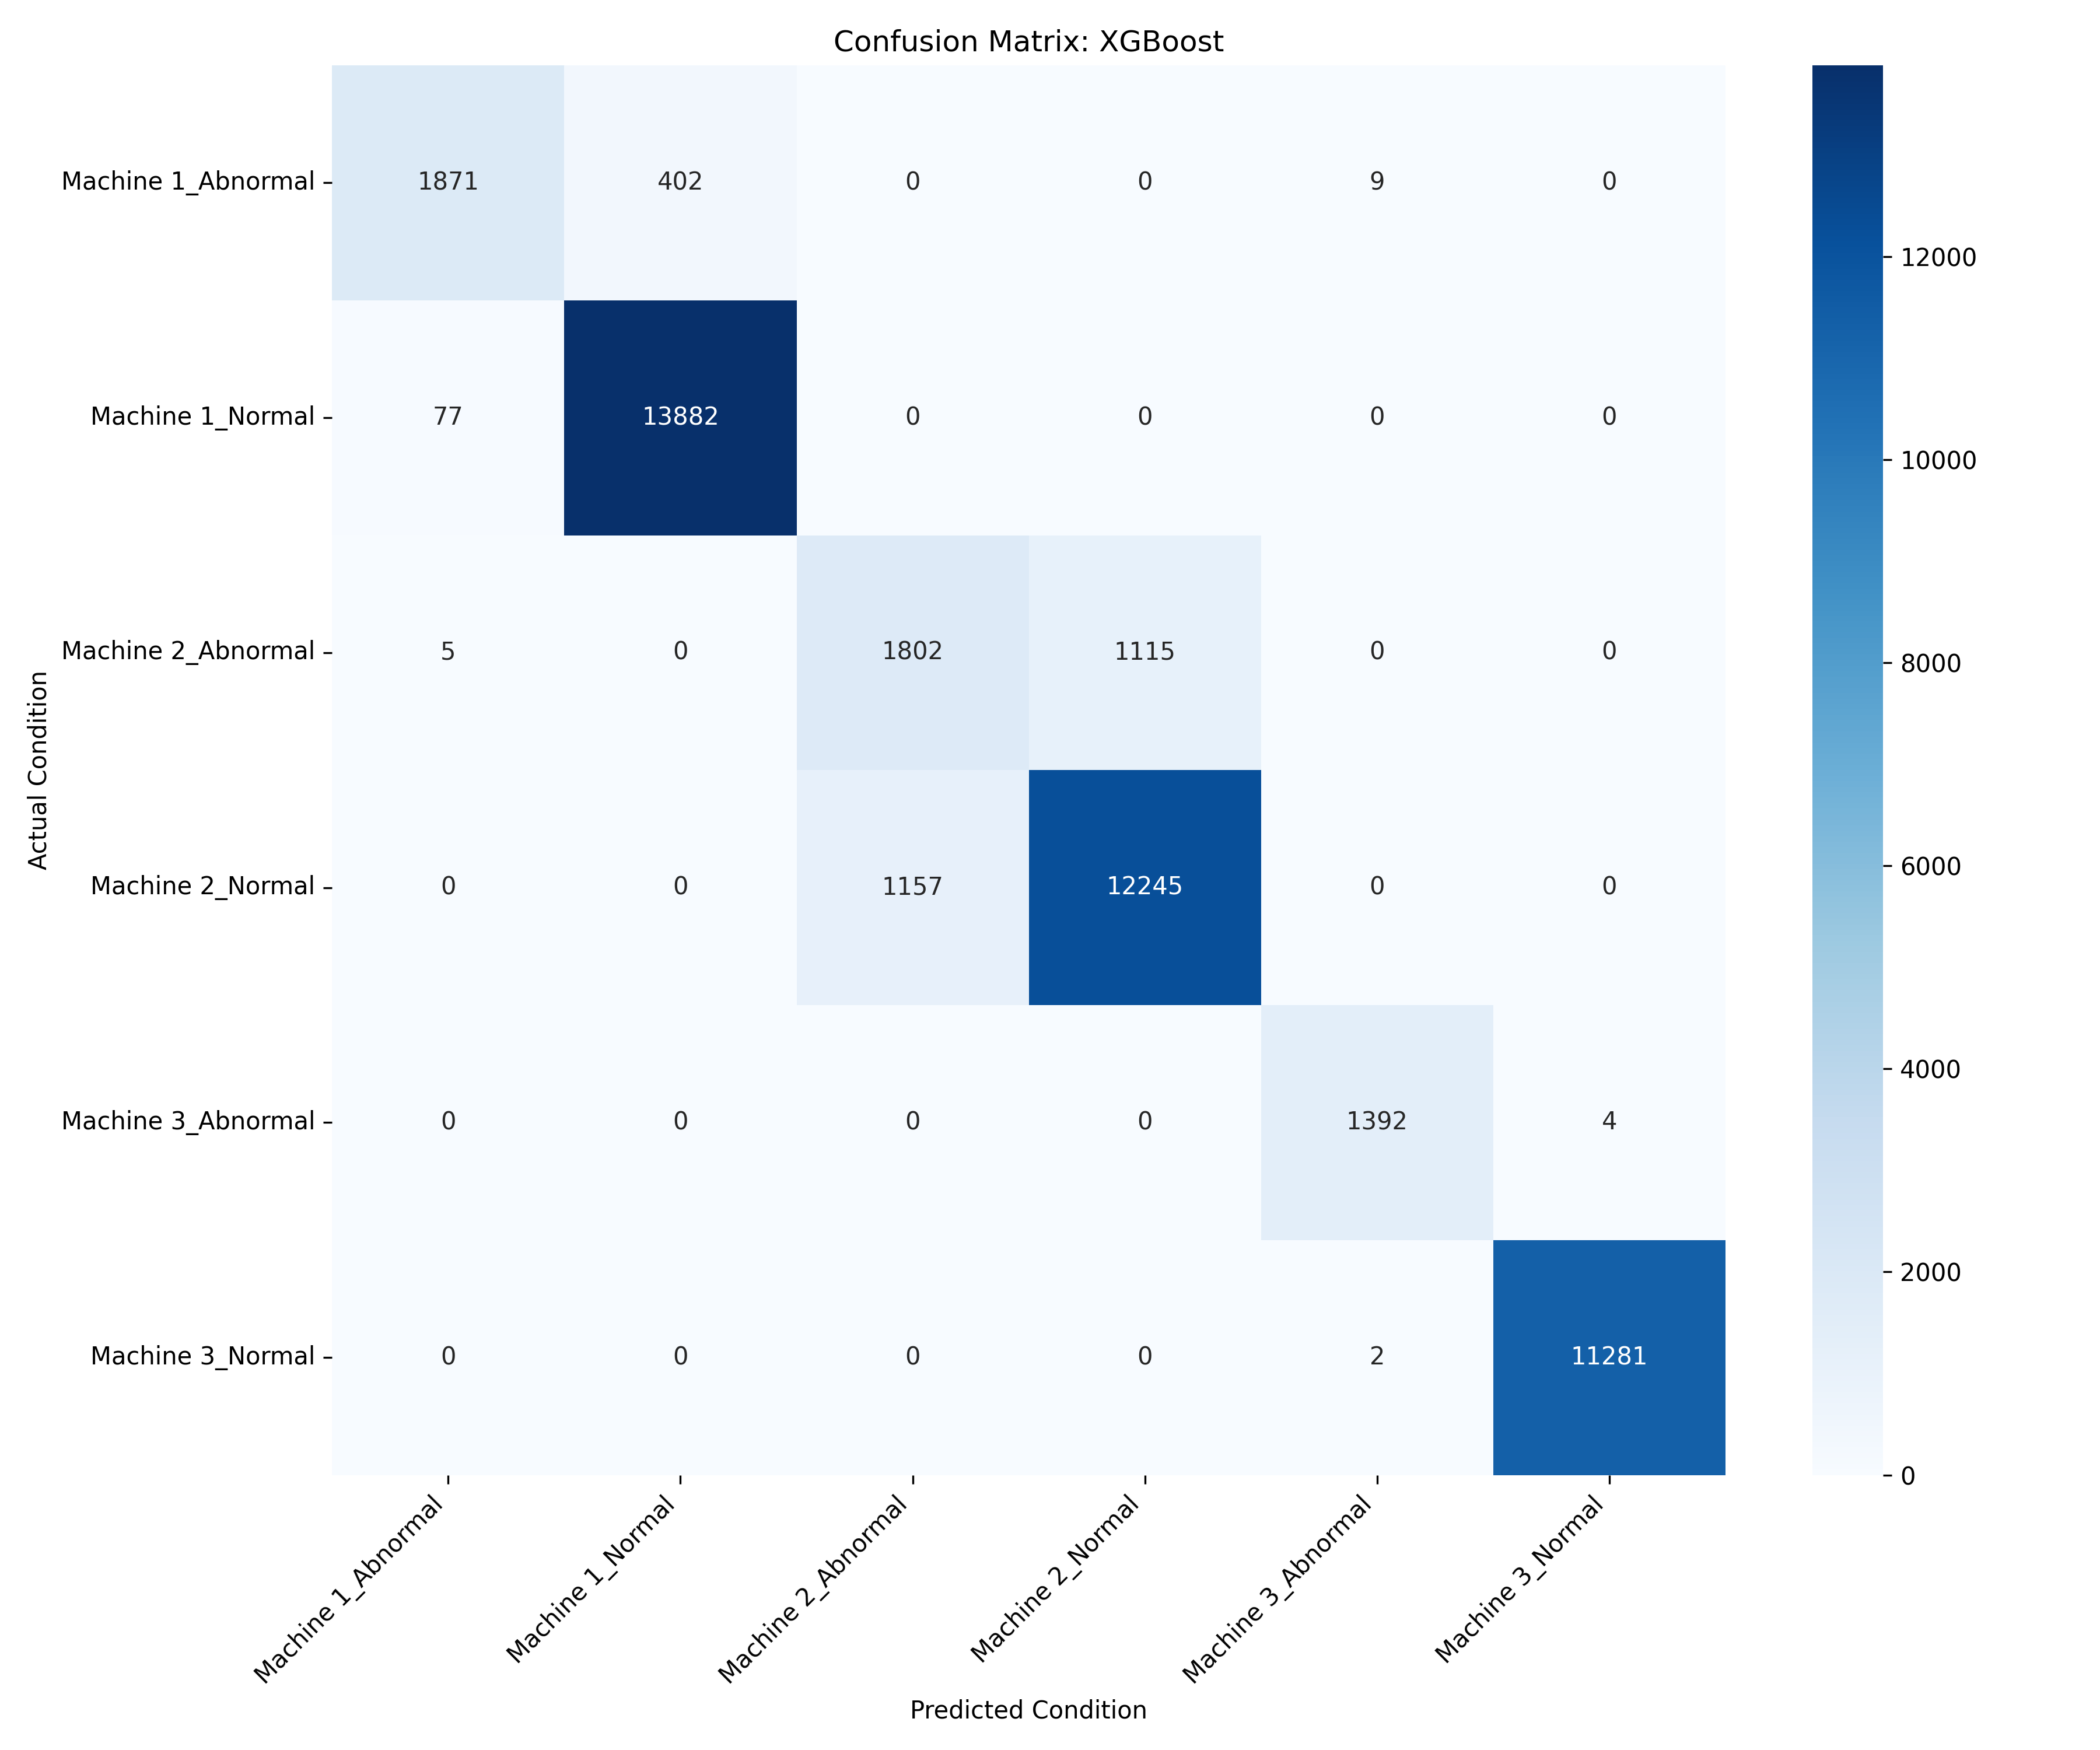
\includegraphics[width=0.8\textwidth]{figures/champion_confusion_matrix.png}
    \caption{Example Diagnostic: Test Set Confusion Matrix}
    \label{fig:conf_matrix}
\end{figure}

These matrices allow engineers to identify specific class-pair confusions (e.g., distinguishing between Machine 1 Normal and Machine 2 Normal) at a glance. Combined with per-class F1-scores, these diagnostics form the basis for our quality assurance gate before any model is promoted to the edge gateways.

\chapter{Conclusion and Future Work}

\section{Project Summary}
This project successfully architected and implemented a high-performance, industrial-grade acoustic anomaly detection system. By transitioning from traditional spectral feature engineering to a sophisticated \textbf{Dual-Track} pipeline, we provided a solution that balances sub-10ms edge inference with deep cloud diagnostics.

Key achievements include:
\begin{itemize}
    \item \textbf{High-Fidelity Diagnostics:} Achieved a validated \textbf{95.61\% test accuracy} and \textbf{0.9267 Macro F1-score} using the \textbf{EfficientAT} architecture, maintaining high precision even under rigorous cluster-aware evaluation.
    \item \textbf{Edge Performance:} Developed a native Rust feature extraction engine (\texttt{fast\_features}) providing a \textbf{57x speedup} over standard libraries, enabling a \textbf{9.8 ms} end-to-end pipeline latency for edge-based XGBoost inference.
    \item \textbf{Generative Data Augmentation:} Addressed critical industrial class imbalance by synthesizing high-fidelity abnormal signatures via a \textbf{Conditional GAN (CGAN)}, boosting minority class F1-scores by over 12\%.
    \item \textbf{Generalized Robustness:} Eliminated recording session bias through a \textbf{DBSCAN Cluster-Aware} evaluation regime, ensuring the system generalizes to new factory environments.
\end{itemize}

\section{Key Takeaways}
The defining success of this project was the resolution of the "Generalization Trap." By treating recording session bias as a manifold clustering problem rather than a standard classification task, we moved beyond superficial high-accuracy metrics to a truly robust system. The deployment of a hybrid architecture—leveraging the speed of gradient-boosted trees for continuous monitoring and the depth of temporal-attention networks for diagnostic deep-dives—represents a state-of-the-art approach to industrial IoT monitoring.

\section{Future Work}
\begin{itemize}
    \item \textbf{Federated Learning:} Implementing a federated training framework to allow models to learn from across multiple factory sites without exposing sensitive acoustic data, improving global robustness while maintaining local privacy.
    \item \textbf{Unsupervised Outlier Exposure:} Integrating an unsupervised branch (e.g., Variational Autoencoders) to detect "zero-day" mechanical failures that were never seen during the training phase.
    \item \textbf{On-Device Quantization:} Utilizing INT8 quantization and ONNX Runtime to deploy the EfficientAT diagnostic model directly onto ARM-based edge gateways, reducing the dependency on cloud connectivity.
\end{itemize}


\backmatter
% \bibliographystyle{plain}
% \bibliography{references}

\end{document}
